%% 
%% Libro en español
%% Pantilla Latex para estructura de un libro en español
%% Autor: Dario A. Palminio
%% LaTeX versión: 2.0
%% Sistema operativo: Ubuntu
%% Editor usado: LaTeXila 2.4.0
%% 

% Document pattern and general formatt
\documentclass[10pt]{book}

% Imports
\usepackage[T1]{fontenc}
\usepackage[utf8]{inputenc} % file charset=utf-8
\usepackage{lmodern}
\usepackage{graphicx} % figuras
\usepackage{subfigure} % subfiguras
\usepackage{hyperref} % To Writing URLs in latex

% Image location (all images into document should be in this location)
\graphicspath{ {images/} } 

% Rename names to spanish language
\renewcommand{\contentsname}{Índice}
\renewcommand{\chaptername}{Capítulo}
\renewcommand{\bibname}{Bibliografía} % Bibliography in spanish
\renewcommand{\figurename}{Figura}
\renewcommand{\listfigurename}{Lista de figuras} 
\renewcommand{\listtablename}{Tablas}

% Page formatt (page size and margins)
%
% Reference: https://es.sharelatex.com/learn/Page_size_and_margins

% Use in main page the following commands:
% \documentclass[10pt]{book} % at start of page
% % Page formatt (page size and margins)
%
% Reference: https://es.sharelatex.com/learn/Page_size_and_margins

% Use in main page the following commands:
% \documentclass[10pt]{book} % at start of page
% % Page formatt (page size and margins)
%
% Reference: https://es.sharelatex.com/learn/Page_size_and_margins

% Use in main page the following commands:
% \documentclass[10pt]{book} % at start of page
% \include{content/page_format} % to include this configuration file

% Formatt:
% Page: 14 x 21 cm
% - margin top and bottom: 2,54 cm
% - margin left and right: 1,91 cm 

\usepackage{geometry}
 \geometry{
 papersize={140mm,210mm},
 left=20mm,
 right=20mm,
 top=25mm,
 bottom=25mm,
 }
 
 
 % to include this configuration file

% Formatt:
% Page: 14 x 21 cm
% - margin top and bottom: 2,54 cm
% - margin left and right: 1,91 cm 

\usepackage{geometry}
 \geometry{
 papersize={140mm,210mm},
 left=20mm,
 right=20mm,
 top=25mm,
 bottom=25mm,
 }
 
 
 % to include this configuration file

% Formatt:
% Page: 14 x 21 cm
% - margin top and bottom: 2,54 cm
% - margin left and right: 1,91 cm 

\usepackage{geometry}
 \geometry{
 papersize={140mm,210mm},
 left=20mm,
 right=20mm,
 top=25mm,
 bottom=25mm,
 }
 
 
 % Page format configuration to 14 x 21 cm

\begin{document}

% General structure

%%%%%%%%%%%%%%%%%%%%%%%%%%%%%%%%%%%%%%%%%%%%%%%%%%%%%%%%%%%%%\
%%%% Author & title page info

% Book's title and subtitle
\title{\Huge 
    \textbf{Ingeniería y Gestión de Proyectos con Scrum}  \\ 
    \huge 
    }

% Book's author
\author{Dario Palminio}

% Book's date
\date{2015} 

\maketitle

            % Title and author
%% 

\tableofcontents
\newpage
\listoffigures
%%\newpage
%%\listoftables
         % contents table and figures list

% Chapters
\chapter{Introducción}

\section{Consideraciones iniciales}

\subsection{Definición}

Scrum es un marco de trabajo (framework) para construir y mantener productos complejos \cite{SBOK-2013} \cite{Scrum-Alliance-2015}. 
Scrum funciona como una implementación del ciclo de mejora continua de Deming (PDCA) y como una implementación de los principios ágiles y principios Scrum. Hay que tener en cuenta que Scrum no es exactamente un proceso íntegro, metodología completa o una técnica para construir productos; sino que, es un marco de trabajo dentro del cual se pueden emplear varias técnicas y procesos \cite{Agile-Atlas-2012}. 

\subsection{Sobre si es una Metodología}

Hay quienes consideran que Scrum no es una metodología, entre otras cosas porque no especifia exactamente el cómo se hacen las cosas, 
sino que dice el qué hacer. Sin embrargo, hay autores y guías que tratan a Scrum como metodología \cite{SBOK-2013}. De hecho en el informe original de Ken Schwaber se habla de metodología \cite{Ken-Schwaber-1995}. En consecuencia, se puede encontrar en numerosa bibliografía que el marco de trabajo Scrum puede ser denominado Metodología de Desarrollo Scrum o Metodología de Gestión de Proyectos Scrum. 
En el primer caso puede deberse a que se puede considerar una metodología como un proceso de desarrollo iterativo e incremental de productos \cite{Ken-Schwaber-1995}. Y en el segundo caso porque se puede considerar que es una alternativa a la gestión clásica de proyectos propuesta por metodologías como la Metodología de Gestión de Proyectos PMI. En este último sentido podemos recordar la definición original de Ken Schwaber: "Scrum es una metodología de gestión, mejora y mantenimiento de un sistema existente o prototipo de producción" \cite{Ken-Schwaber-1995}.
 
Por otro lado, considerando que Scrum define roles, artefactos, actividades, flujo del ciclo de actividades Scrum \cite{Agile-Atlas-2012}, reglas y algunas sugerencias de implementación como, además, al definir el flujo del ciclo de Scrum o flujo de trabajo define parcialmente un cómo, en el cual incluye una secuencia básica de cosas a hacer; por eso, y sin ser puristas, se puede considerar como una forma de metodología de trabajo y de gestión. O sea que puede funcionar como una metodología a alto nivel o plataforma de trabajo sobre la cual pueden funcionar otras metodologías, más específicas de producción y desarrollo, y otras técnicas y procesos. Por este motivo, 
Scrum puede ser adaptado a diversas empresas y organizaciones que trabajen con metodologías diferentes pero compatibles con los 
lineamientos de Scrum (sus valores y principios) y del Movimiento Ágil (filosofía ágil). Se puede usar Scrum y a su vez utilizar técnicas de otras metodologías para implementar sus actividades y sugerencias. O sea que cuando se usa Scrum se hace una aproximación empleando diversas técnicas y, posiblemente, otras metodologías.

\subsection{Ámbito de aplicación}

Relacionado a su ámbito de aplicación se pude decir que Scrum no es un marco de trabajo orientado a implementarse en cualquier dominio y contexto. Scrum está pensado para proyectos bajo "dominios complejos" [Snowden 2007] donde existe un grado alto de incertidumbre y baja predictibilidad (ver figura \ref{fig:MarcoCynefinModel}). O sea que es útil en ámbitos con requisitos inciertos y riesgos técnicos altos. Nos permite encontrar prácticas emergentes en dominios complejos, como por ejemplo en la gestión de proyectos de innovación \cite{Martin-Alaimo-2014}. Está orientado a contextos que necesitan niveles altos de creatividad, innovación, interaccion y comunicación. Por este motivo, es bastante empleado en la industria de software, ya que en la misma existen contextos específicos de alta complejidad e incertidumbre con necesidad de creatividad e innovación. Pero también se utiliza en otras industrias con dominios de problemas de complejidad semejante. Por ejemplo ha sido empleado en: educación, organizaciones de campañas publicitarias, industria de productos de innovación, empresas de editoriales de libros, etcétera.

\begin{figure}[h]
  \centering
  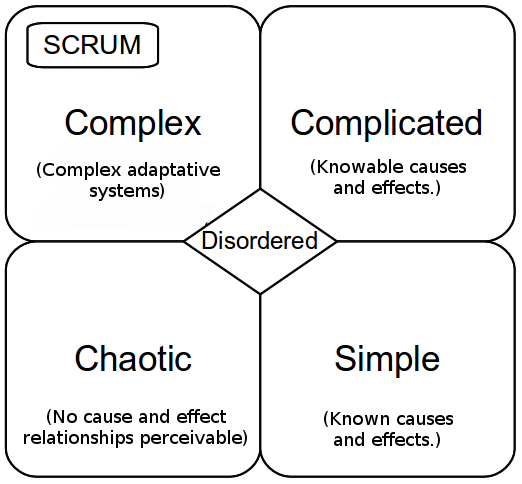
\includegraphics[width=0.50\textwidth]{MarcoCynefinModel}
  \caption{Modelo de dominios de Marco Cynefin}
  \centering
  \label{fig:MarcoCynefinModel} %\ref{fig:MarcoCynefinModel}
\end{figure}

\subsection{Visión general}

En esta metodología se definen los principios y valores a seguir, los roles, relaciones y respnsabilidades, los artefactos o entidades manejadas en el proceso de trabajo, un conjunto de reuniones o actividades en un flujo de trabajo como resume la imagen de la figura \ref{fig:ScrumMapMind}.

\begin{figure}[h]
  \centering
  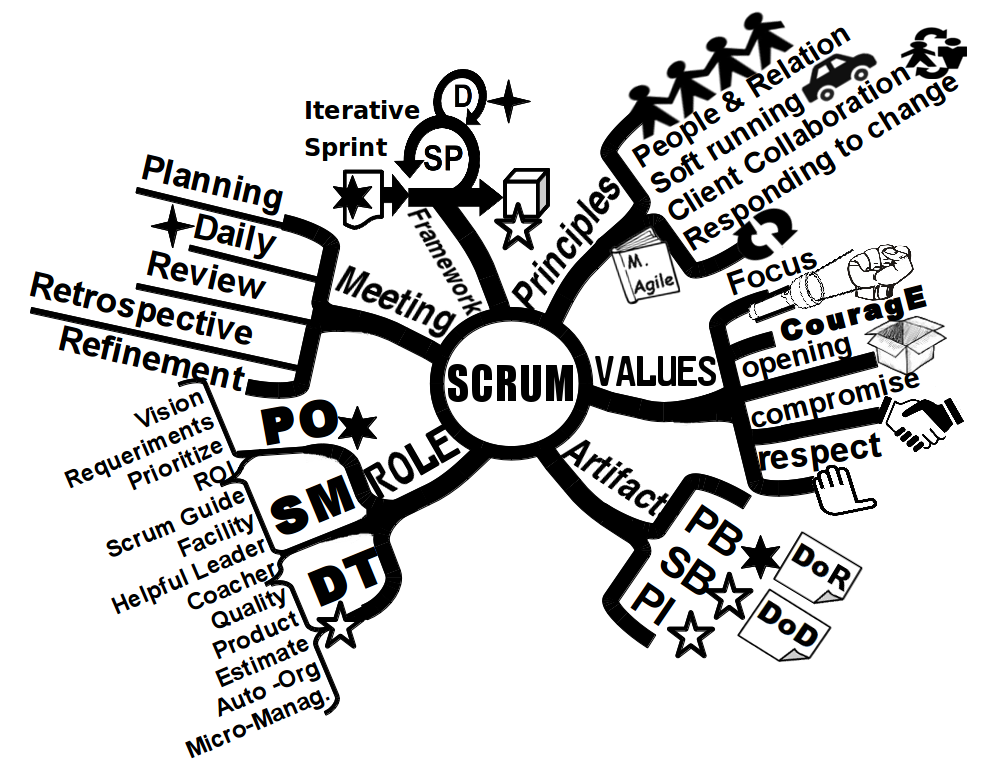
\includegraphics[width=0.99\textwidth]{ScrumMapMind}
  \caption{Mapa mental sobre Scrum}
  \centering
  \label{fig:ScrumMapMind} %\ref{fig:ScrumMapMind}
\end{figure}

En los siguientes capítulos se explicarán los diferentes aspectos y características de la propuesta de este marco de trabajo con lo que 
al final del libro el mapa mental de la figura \ref{fig:ScrumMapMind} quedará explicado y será fácilmente entendible. 
     % Initial considerations
\chapter{Origen}

\section{Origen histórico}

El origen de Scrum se remonta a la década del 80. La revista gerencial "Harvard Business Review" publica un artículo de Takeuchi y Nonaka denominado: "El nuevo nuevo juego para el desarrollo de productos" \cite{Takeuchi-Nonaka-1986}. En el artículo se describe cómo empresas tales como Honda, Canon y Fuji-Xerox producían nuevos productos a nivel mundial utilizando un enfoque diferente al tradicional de entonces. En ese artículo se introdujo el concepto Scrum, con el término tomado del deporte Rugby, para simbolizar este nuevo enfoque basado en equipos integrales para el desarrollo de productos.

Una década más tarde, Jeff Sutherland y su equipo en Easel Corporation crearon el proceso de Scrum para ser utilizado en los procesos de 
desarrollo de software tomando los conceptos del artículo original de Takeuchi y Nonaka. Luego, en 1995, Jeff Sutherland junto con Ken Schwaber publican un informe sobre Scrum en una conferencia de Programación Orientada a Objetos OOPSLA. El informe fue formalizado con el nombre Proceso de Desarrollo SCRUM \cite{Ken-Schwaber-1995}. Desde esa fecha, Schwaber and Sutherland, han producido y publicado varias especificaciones para Scrum que han servido como guías y material de referencia.

Luego, en los 90, Scrum paso a ser reconocidamente parte de las llamadas "Metodologías de Desarrollo de Software de peso liviano", junto a Crystal (1992), Feature Driven Development (1997), Desarrollo de Software Adaptativo (1999) y Extreme Programming (1999). Y luego del Manifiesto Ágil \cite{Beck-2001}, promulgado en 2001 y firmado por Ken y Jeff, pasó a ser reconocida como parte del movimiento ágil y su filosofía. Ken Schwaber fue el primer presidente de la Alianza Ágil fundada tras el Manifiesto Ágil.

Desde que surgió se popularizó en en el mundo industrial, principalmente en la industria de software, miles de proyectos en todo el mundo han utilizado Scrum para el desarrollo de productos, tanto en empresas pequeñas (startups) como en multinacionales. Debido a su amplia aplicación surgieron diferentes entidades capacitadoras y certificadoras para difundir Scrum y certificar el conocimiento de quienes rinden los respectivos exámenes necesarios. La Scrum Alliance \cite{Scrum-Alliance-2015} es un ejemplo de este tipo de organizaciónes y es considerada una de las principales reconocidas certificantes. La Scrum Alliance fue fundada en 2002 por Ken Schwabe, Mike Cohn y Esther Derby. En 2006, Jeff Sutherland creó su propia compañía llamada Scrum.inc, sin dejar de ofrecer y enseñar a los cursos de Certified Scrum.
Ken dejó la Alianza Scrum en 2009 para fundar la Scrum.org para mejorar aún más la calidad y la eficacia de Scrum, principalmente a través de la serie Profesional Scrum ("Professional Scrum series").

\section{Origen causal}

Scrum tuvo un origen causal que suele constituir el análisis crítico previo a su explicación. Scrum emerge del intento de resolver un problema y de la crítica a las consideradas causas del mismo. Scrum vino a surgir como una alternativa al modo en que se desarrollaba software y lo hizo como posible solución a los problemas que presentaba la situación en ese entonces (década del 90) de Desarrollo de Software. Por esa razón es que por lo general cuando se habla de Scrum se hace un análisis crítico previo para plantear un cambio debido a un problema. Por un lado, Scrum plantea un cambio paradigmático o filosófico que consiste en un cambio de perspectiva y de mentalidad (mindset). La otra cuestión fundamental es la metodológica en la cual se propone un cambio del proceso de desarrollo de software o proceso industrial de software. Por este motivo, para comenzar a comprender Scrum, hay que comprender cuál es el problema que viene a intentar resolver y qué es lo que se critica.

\subsection{Problema}

El problema principal por el que Scrum surgió como alternativa consistió en que la mayoría de los proyectos de desarrollo de software no lograban entregarse en tiempo, dentro de los costos y con las funcionalidades comprometidas. Ya en la primera conferencia organizada por la OTAN (en 1968) sobre desarrollo de software se hablaba de la "Crisis del Software" haciendo mención de los problemas recurrentes en que se veía afectado el desarrollo de software y sus resultados. En ese momento se identificaron entre diversos problemas la baja calidad del software que se desarrollaba, el no cumplimiento de las especificaciones y el código prácticamente inmantenible que dificultaba la gestión y la evolución de los proyectos. Una encuesta de cientos de proyectos de desarrollo de software empresarial indicó que cinco de seis proyectos de software se consideraban no satisfactorios \cite{AntiPatterns-1998}, por otro lado sólo 29 de cada 100 proyectos de IT se terminaban exitosamente y el 71 por ciento de los clientes no estaban satisfechos con los resultados (Standish Groups Chaos Report 1994 - 2004). En el año 1994 el Standish Group publicó un estudio conocido como el "CHAOS Report" \cite{CHAOS-Report-1994} donde se mostró las siguientes tasas de fracaso en los proyectos de desarrollo de software en general:

\begin{itemize}

\item \textbf{Proyectos cancelados:} el 31.1 por ciento es cancelado en algún punto durante el desarrollo del mismo.
\item \textbf{Proyectos insuficiente:} el 52.7 por ciento es entregado con sobrecostos, en forma tardía o con menos funcionalidades de las inicialmente acordadas.

%Las conclusiones de la investigación sugieren que el involucramiento del usuario y el empleo de periodos de tiempo más cortos son claves para incrementar las tasas de proyectos exitosos

\end{itemize}

\subsubsection{Causas}

Los problemas detectados en los modelos tradicionales se fundamentan principalmente en lo siguiente: 

\begin{itemize}

\item \textbf{Entorno cambiante:} Entorno altamente cambiante propio de la industria \cite{Martin-Alaimo-2014}.

\item \textbf{Dependencia de Procesos rígidos:} el proceso mismo de desarrollo de software donde el resultado depende de la actividad
cognitiva de las personas más que de las prácticas y controles empleados \cite{Martin-Alaimo-2014}. Las metodologías de desarrollo de software resultaron muy pesadas y prohibitivas para responder satisfactoriamente a los cambios de negocio.

\end{itemize}

\subsection{Filosofía criticada}

Como se dijo antes, con Scrum se plantea un cambio paradigmático o filosófico que consiste en un cambio de perspectiva y de mentalidad (mindset).

\subsection{Metodología criticada}

La causa de los problemas y fracasos de los proyectos de software en la situación dada, en ese entonces, de Desarrollo fueron atribuidos principalmente a la Metodología Cascada (Waterfall Methodology) \cite{Ken-Schwaber-1995}. Pero hay que tener en cuenta de qué se habla cuando se critica a la metodología cascada. Pues la metodología cascada no es el modelo cascada y en ocaciones se han atribuido, en un sentido erróneo, las causas de los problemas al modelo cascada. Pues no se puede comparar Scrum con el modelo Cascada porque Scrum no es exactamente un modelo y ofrece soluciones a aspectos que el modelo cascada no ofrece. Aunque si, el modelo cascada, es perte de lo que se podría considerar una Metodología Cascada. 

\subsubsection{Modelo en Cascada}

El Modelo en Cascada (Waterfall Methodology) \cite{Ken-Schwaber-1995} es un Modelo Secuencial de Procesos para la ingeniería de software presentado por Winston Royce en 1970, aunque ya se venía desarrollando desde antes. Para algunos críticos, el Modelo en Cascada, se convirtió en el modelo metodológico más utilizado dentro de la industria en un período de tiempo. Pero hay que considerar que el modelo solo abarca al sistema de producción o sistema de desarrollo (ver "Development Process" en la figura \ref{fig:WaterfallMethodology}) de la industria y no al de gestión.

En un sentido lato y ortodoxo se puede decir que el Modelo en Cascada refleja un proceso lineal y secuencial de un conjunto de procesos o fases independientes dentro de un proyecto. Las fases son: requerimientos (requerimiento del sistema y requerimientos del software), diseño, codificación, pruebas y operación. Según esto y siempre cuando el proceso de desarrollo de un proyecto conste de solo la secuencia de estas fases sin repetición, la principales críticas como desventajas que se hacen son:

\begin{enumerate}

\item \textbf{Previción:} Al tener una face de requerimientos única al comienzo, el producto final es anticipado de antemano \cite{Scrum-Institute-2015}. Esto requiere de cierta previción y certidumbre inicial que en proyectos complejos y cambiantes es poco factible que suceda.

\item \textbf{Requerimientos no necesarios:} Requerimientos elicitados al comienzo del proyecto y luego implementados nunca serán completamente necesitados por el cliente \cite{Scrum-Institute-2015}. O sea que pueden haber requerimientos irrelevantes o inecesariamente implementados, ya sea porque el cliente dejó de tener la necesidad en el transcurso del proyecto o porque la incertidumbre inicial generó una mala elicitación de los mismos.

\item \textbf{Fases separadas:} Cada fase es estrictamente separada \cite{Scrum-Institute-2015}. Por ejemplo una vez que se encuentra completa la fase de requerimientos se procede a una firma de aprobación o "sign-off" que congela dichos requerimientos, y es recién aquí cuando se puede iniciar la fase de diseño, fase donde se crea un plano de modelo o "blueprint" del mismo para que, luego, los programadores lo codifiquen y se prosiga con las pruebas y finalmente el despliegue en operación. Pues en entornos altamente cambiante, propio de la industria de software, esta forma secuencial estricta hace del proceso de desarrollo un proceso “pesadas” (estanco y burocrático) y prohibitivo para responder satisfactoriamente a los factores cambiantes de negocio \cite{Martin-Alaimo-2014}.
%Solución propuesta por scrum:
%Fine-grained requirements are only defined when they are really needed.
%All activities to design, build and test a certain functionality are kept together in one phase.
%Changes are expected and welcomed by Scrum team.

\end{enumerate}

\subsubsection{Gestión de Proyectos Clásica}

\subsubsection{Metodología en Cascada}

\begin{figure}[h]
  \centering
  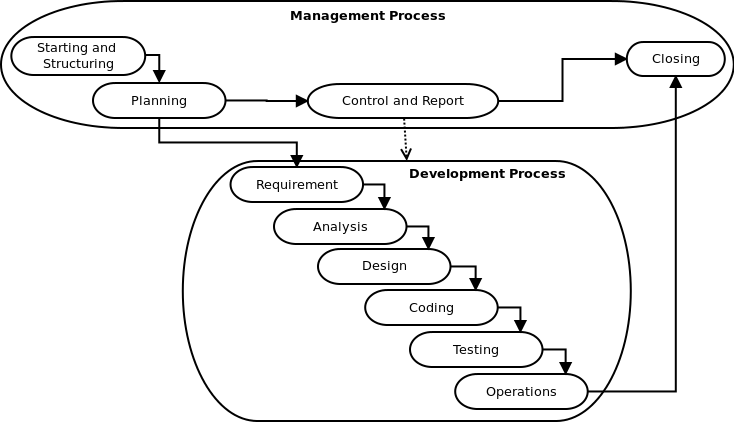
\includegraphics[scale=0.5]{WaterfallMethodology}
  \caption{Metodología Cascada criticada (Diagrama integrador del Modelo Cascada \cite{Winston-Royce-1970}, la Metodología Cascada \cite{Ken-Schwaber-1995} y la Metodología de Gestión de Proyectos \cite{PMBOK-1996})}
  \centering
  \label{fig:WaterfallMethodology} %\ref{fig:WaterfallMethodology}
\end{figure}
           % Origin and previous critical analysis
\chapter{Filosofía Scrum}

Discriminando todas las filosofías generales, como ideologías y concepciones religiosas, podemos decir que hay filosofías relacionadas específicamente al desarrollo de sistemas y de software. Pues, si bien ocurre que ideologías políticas influyen en los desarrolladores, líderes y arquitectos hay ideas más a fines del ámbito de desarrollo de sistemas, ideas que podemos decir que conforman filosofías influenciadoras. Estas influencias son notorias cuando vemos que se toma una decisión de usar una determinada metodología que implementa determinados principios o seguir determinados principios sin datos empíricos que sostienen su uso ni explicaciones racionales soportadas con evidencia. A veces dichos principios son como sacados de la galera o reflejan expresión de deseos. Tal como sucede cuando se aplican determinadas tecnologías o metodologías como si se tratasen de una moda o de algo aparentemente arbitrario. También esto se puede apreciar cuando escuchamos decir en una reunión de trabajo en equipo que se premiará al individuo que sobresale (filosofía individualista), que “el éxito del grupo está por encima del individual” (filosofía Ubuntu o cooperativa), escuchamos en una reunión técnica que “el software debe ser libre” (filosofía Free Software) o que solo se desarrollara software propietario, que “las mejores arquitecturas, requisitos y diseños emergen de equipos autoorganizados” \cite{Beck-2001} (filosofía ágil); o que “el software es un mundo de objetos” (filosofía del Paradigma Orientado a Objetos). Las consignas o lemas organizacionales, los mantras personales o institucionales, las visiones empresariales y lineamientos institucionales también son, en muchos casos, una expresión de filosofías que condicionan a las personas y al desarrollo de software. Por ejemplo, en particular, se da con las filosofías del pensamiento sistémico, pensamiento crítico, filosofía ágil, software libre, software abierto o software propietario, que son las principales que en el mundo del desarrollo de software influencian a sus actores. Estas filosofías suelen presentar principios a seguir y estos principio guían algunas metodologías (prácticas y métodos) de desarrollo de sistemas y a gran parte de desarrolladores de sistemas. Aquí nos vamos a centrar en la filosofía Scrum y la filosofía Ágil.

\section{Mentalidad y modelos mentales}

Las personas que participan en el desarrollo de sistemas, diseños organizacionales o industrias de software tienen experiencias, creencias, principios, vivencias y valores que repercuten y condicionan el modo en que ellas perciben la realidad de su día a día y, en consecuencia, repercuten y condicionan su actuar, su forma de hacer, su trabajo y el resultado del mismo, sistemas hombre-máquina o software. Estas ideas, en los gerentes y desarrolladores, son modelos mentales que conforman una mentalidad, o lo que se denomina mindset (Masa Maeda 2012 \footnote{Masa K Maeda es PhD, Founder and CEO de Valueinnova USA (capacitación Scrum). Es el creador de Serious LeAP, consultor senior del Cutter Consortium en Boston, miembro del comité de dirección del Agile Testing Alliance y maestro en la Universidad de California en Berkeley. Es pionero de Lean y Kanban para trabajo de conocimiento y uno de los formadores del Lean Kanban University. Es una figura líder mundial en Agile y ha generado Serious Games de alto calibre. Previamente hizo I+D para Apple Inc en USA y para Justsystems en Japón. Obtuvo el doctorado y la maestría en Japón.}). O sea que la filosofía que una persona siga o adhiera está relacionada a los modelos mentales de esa persona y forja su mentalidad o mindset que en algún sentido lo guía.

Los modelos mentales pueden definirse como: “imágenes internas, que están profundamente arraigadas, de cómo funciona el mundo, imágenes que nos limitan a las formas familiares de pensar y actuar”. Los modelos mentales abarcan cuestiones acerca de cómo vemos el mundo y de cómo actuamos en el mundo. 

Tener noción de los modelos mentales es importante para entender que hay detras de las acciones, detras de las prácticas y de las metodologías usadas. Nos ayuda a comprender que para realizar cambios en las acciones de las personas y cambios en la forma de hacer las cosas es necesario, la mayoría de las veces, cambiar la mentalidad. Sin cambio de mentalidad puede hacerse insostenible en el tiempo un cambio de hábito, práctica o metodología. Por ese motivo, seguir principios en forma mecánica o por ovediencia a la autoridad no forma convicción, y seguir una filosofía sin convicción es un primer condicionante de fracaso práctico en su implementación.

\section{Principios}

En la industria de sistemas y software los principios son reglas, proposiciones o normas que funcionan como máximas o preceptos que orientan la acción. O sea que un principio es como “una regla general de conducta o comportamiento” \cite{Lawson-Martin-2008} \cite{SEBoK-2014}. Un principio es como una recomendación sin el cómo se sigue la recomendación. Cómo hará para seguir la recomendación depende de usted o de quien decida seguir el principio. Por eso son la base, origen y razón fundamental sobre la cual se procede o discurre en materia de sistemas. Se suele usar en el contexto de procesos de desarrollo y metodologías como proposición que da razón, punto de partida o guía, como fundamento de un conjunto de prácticas, una metodología o paradigma de trabajo siendo las metodologías las encargadas de definir el cómo se implementan.

Cada uno sigue algunos principios en su vida como: "trabajo colaborando". También seguimos principios éticos como: “nunca mentir” o “no robar”. A semejanza de los principios éticos tradicionales, ocurre que los principios no necesariamente tienen fundamento objetivo, racional, empírico o basado en evidencias; pues, en ocasiones se comportan más como principios filosóficos que como principios científicos. Lo cual no quiere decir que no deba buscarse que los principios en ingeniería no sean sacados de la galera o usados de forma irracional, sin justificativo razonable y sin comprobación. Es preferible aplicar principios de comprobada efectividad en su aplicación. El aplicar principios comprobados reduce la cantidad de tiempo necesaria para crear las salidas de planificación de los recursos humanos y mejora la probabilidad de que la planificación sea efectiva \cite{PMBOK-2004}, del mismo modo aplicar principios comprobados en actividades de desarrollo y diseño de sistemas reduce tiempos de investigación para generar la salida deseada y minimiza riesgos, mejorando la probabilidad de que el desarrollo sea efectivo. 

Los principios de Scrum son las pautas básicas para aplicar el marco de Scrum y guía a usarse en todos los proyectos Scrum \cite{SBOK-2013}, proyectos en los que se aplica metodología Scrum. Los principios de Scrum se orientan a la gestión de proyectos, desarrollo de productos, trabajo en equipo y el trabajo en base a los principios ágiles. O sea que los principios Scrum tienen correlación con los principios ágiles en forma prácticamente directa \cite{Agile-Atlas-2012}. Y los principios de Scrum están alineados a los valores de Scrum que son: Foco, Coraje, Apertura, Compromiso y Respeto.


A continuación se describen los principios y valores del Manifieto Ágil y de Scrum.

\section{Manifiesto Ágil}

Los principios del desarrollo ágil se encuentran en el Manifiesto por el Desarrollo Ágil de Software o Manifiesto Ágil [Manifesto Agile 2001], el que expone valores y principios firmado por diecisiete personas convocadas por Kent Beck \cite{Beck-2001}. Los principios del desarrollo ágil surgieron como principios base y originarios de métodos que estaban surgiendo como alternativa a las metodologías clásica formales (CMMI, SPICE, etc.) a las que, autores como Kent Beck, consideraban excesivamente pesadas y rígidas por su carácter normativo y fuerte dependencia de planificaciones detalladas completas y previas al desarrollo \cite{Wiki-2015}.

\subsection{Valores del Manifiesto Ágil}

El Manifiesto Ágil propone los siguientes valores:

\begin{enumerate}

\item \textbf{Individuos e interacciones sobre procesos y herramientas:} hay que priorizar la confianza puesta en los equipos, los individuos dentro de esos equipos y la manera en que éstos interactúan en vez de seguir rígidamente procesos y herramientas. Pues, son los equipos quienes deben resolver qué hay que hacer, cómo hay que hacerlo y finalmente son ellos quienes lo hacen. Pues los equipos no deberán ser meros autómatas que reciben órdenes jerárquicas de la organización de arriba hacia abajo sino que, en lugar de eso, se espera que de abajo hacia arriba sepan resolver los problemas, ofrecer sus propios métodos de trabajo y ser hasta cierto punto autosuficientes. En este sentido, hay que delegar en ellos la identificación de qué se interpone en el camino de sus metas y la asunción de la responsabilidad de resolver todas las dificultades que se encuentren dentro de su alcance. Se les debe permitir trabajar en conjunto con otras partes de la organización para resolver asuntos que están más allá de su control.

\item \textbf{Software funcionando sobre documentación extensiva:} hay que estar orientado al producto o focalizarse en él y de este modo requerir un incremento de producto completo y funcionando como resultado final de cada ciclo de trabajo, en vez de tener que cumplir con grandes y engorrosas documentaciones y formalismos burocráticos. Ciertamente, en la construcción del producto, sea necesario realizar determinada documentación, pero es el producto concreto o funcionando lo que permite a la organización guiar al proyecto hacia el éxito. Es crucial que los equipos produzcan un incremento de producto en cada ciclo de trabajo.

\item \textbf{Colaboración con el cliente sobre negociación contractual:} en vez de tener comunicación pobre debido a restricciones contractuales, el cliente debería ser el punto de contacto principal del equipo, en colaboración de trabajo, con los eventuales usuarios finales del producto y con las partes de la organización que necesitan el producto. Se debería ver al cliente como un miembro del equipo que trabaja colaborativamente con el resto de integrantes para decidir qué debe hacerse y qué no. Con el cliente se debería poder seleccionar el trabajo que debe realizarse a continuación, asegurando que el producto tenga el valor más alto posible en todo momento. Esto es crucial construir una fuerte colaboración con el cliente en vez de negociar contratos rígidos que obstaculizan el trabajo ágil y generan fricción con el cliente.

\item \textbf{Respuesta ante el cambio sobre seguir un plan:} el avance del trabajo o del equipo debería estar representado por un incremento de producto real y que funciona, y no por una correcta correlación y contrastación a un plan. Se debe priorizar la flexibilidad para adaptación a cambios en vez de la rigidez de seguir un plan detallado. Para ello, los equipos deberían inspeccionar lo que sucede de forma abierta y transparente buscando adaptar sus acciones a la realidad. O sea que, la planificación se debería adaptar a la realidad y al equipo y no al revés.

\end{enumerate}

Se puede notar que estos valores son aplicables a cualquier tipo de organización e industria. Pues, solo el segundo valor se refiere particularmente a la industria de software y el mismo se puede reformular de forma más general como sigue: trabajar orientados al producto funcionando más que sobre una amplia y extensa documentación \cite{Sriram-Narayan-2015}.

\subsection{Principios del Manifiesto Ágil}

Alineados a estos valores, el Manifiesto Ágil propone los siguientes principio:

\begin{enumerate}

\item \textbf{Entregar valor temprano y continua:} Nuestra mayor prioridad es satisfacer al cliente mediante la entrega temprana y continua de software con valor (alineado al principio de "entregar lo más rápido posible" de Lean).

\item \textbf{Apertura al cambio:} Aceptamos que los requisitos cambien, incluso en etapas tardías del desarrollo. Los procesos Ágiles aprovechan el cambio para proporcionar ventaja competitiva al cliente.

\item \textbf{Entregables frecuentes:} Entregamos software funcional frecuentemente, entre dos semanas y dos meses, con preferencia al periodo de tiempo más corto posible (alineado al principio de "entregar lo más rápido posible" de Lean).

\item \textbf{Cooperación con el cliente:} Los responsables de negocio y los desarrolladores trabajamos juntos de forma cotidiana durante todo el proyecto (alineado al principio de "potenciar al equipo" de Lean). O sea que se privilegia una cooperación constante entre miembros del equipo e interesados externos al equipo (como clientes).

\item \textbf{Personas motivadas:} Los proyectos se desarrollan en torno a individuos motivados. Hay que darles el entorno y el apoyo que necesitan, y confiarles la ejecución del trabajo (alineado al principio de "entregar lo más rápido posible" de Lean).

\item \textbf{Conversación cara a cara:} El método más eficiente y efectivo de comunicar información al equipo de desarrollo y entre sus miembros es la conversación cara a cara.

\item \textbf{Orientación al producto:} El software funcionando es la medida principal de progreso.

\item \textbf{Desarrollo sostenible:} Los procesos Ágiles promueven el desarrollo sostenible. Los promotores, desarrolladores y usuarios debemos ser capaces de mantener un ritmo constante de forma indefinida.

\item \textbf{Excelencia técnica:} La atención continua a la excelencia técnica y al buen diseño mejora la Agilidad.

\item \textbf{Simplicidad eficiente:} La simplicidad, o el arte de maximizar la cantidad de trabajo no realizado, es esencial (alineado al principio de simplicidad). Este estilo de prácticas es parte de algo que, en metodologías ágiles, se conoce como: "hacer todo lo posible por hacer lo menos posible" \cite{Anacleto-2005}. Por ejemplo en Arquitectura se puede considerar mantener una lo más simple posible. Si la simpleza se traduce en facilidad de uso de la arquitectura, facilidad para entender los conceptos involucrados y documentación necesaria, es muy probable que el nivel de productividad aumente \cite{Anacleto-2005}. En este sentido la simpleza de la arquitectura es un requerimiento de calidad alineado a la filosofía ágil.

\item \textbf{Equipos auto-organizados:} Las mejores arquitecturas, requisitos y diseños emergen de equipos auto-organizados (alineado al principio sistémico de emergencia).

\item \textbf{Equipos auto-reflexivos:} A intervalos regulares el equipo reflexiona sobre cómo ser más efectivo para a continuación ajustar y perfeccionar su comportamiento en consecuencia.

\end{enumerate}

\section{Valores de Scrum}

\begin{enumerate}
\item \textbf{Foco:} hay que enfocarse en sólo unas pocas cosas a la vez, trabajamos bien juntos y buscando producir un resultado excelente tratando de entregar ítems valiosos en forma pronta.

\item \textbf{Coraje:} hay que buscar sentirse apoyados y tener más recursos a disposición para promover el coraje para enfrentar desafíos más grandes. Además, para poder lograr cambios significativos en una organización que mantiene una cultura con principios y valores que entran en conflicto con los de Scrum y el Manifiesto Ágil, es necesario tener coraje para impulsar el cambio y plantarse en forma efectiva ante la resistencia al cambio. En este sentido, coraje se refiere al valor que hay que tener para no dejarse dominar ante la idiosincrasia predominante y el “status quo” que atentan contra el pensamiento Scrum.

\item \textbf{Apertura:} Hay que tener apertura para expresar cotidianamente cómo nos va, qué problemas encontramos, manifestar las preocupaciones y aceptar las sugerencias de los pares para que éstas puedan ser tomadas en cuenta por nosotros y por los demás. La apertura requiere capacidad de aceptación y tolerancia ante la crítica y la opinión de los demás.

\item \textbf{Compromiso:} Se busca lograr compromiso para el éxito gracias a promover el mayor control nuestro sobre lo que hacemos y nuestro destino. Hay mayor probabilidad de lograr compromiso en las personas que deciden sobre lo que hacen.

\item \textbf{Respeto:} Buscamos convertirnos en merecedores de respeto a medida que trabajamos juntos, compartiendo éxitos y fracasos, llegando a respetarnos los unos a los otros y ayudándonos mutuamente.
\end{enumerate}

\section{Principios de Scrum}

Se suele asociar a los valores del Manifiesto Ágil como principios de Scrum. Por lo que, en primera instancia, los cuatro valores ágiles son los principales principios de Scrum. Pero para no repetirlos en esta sección vamos a nombrar otros seis principios que en diferente bibliografía se suelen atribuir a Scrum. Los mismos son:

\begin{enumerate}

\item \textbf{Control Empírico:} El proceso empírico de control del proyecto es más efectivo que el control predictivo de largos plazos. Es más efectivo para gestionar la complejidad y obtener el mayor valor posible, basado en inspección y adaptación regular en función de los resultados que se van obteniendo y del propio contexto del proyecto. El proceso empírico permite adaptabilidad a requisitos que emergen del mismo proceso de desarrollo. Con este principio como marco, podemos usar metodologías, prácticas y técnicas, y ser nosotros (o el propio equipo de trabajo) los que a través del empirismo, determinemos la forma más adecuada de hacer las cosas para lograr los objetivos. Son los equipos de desarrollo los que deben hacer lo que sea necesario para entregar el producto esperado y aprender de su propia experiencia mediante exploración y experimentación \cite{UNTREF-2014}. Es el equipo el que determina qué prácticas y herramientas les dan los mejores resultados, y así mejoran de manera continua. Los buenos equipos trabajarán constantemente en mejorar y aprender de sus experiencia. Además, se debe aprender de la experiencia de los demás leyendo libros y buscando la experiencia de personas que ya hayan venido probando algunas prácticas, o que están experimentando con nuevas potenciales mejores formas de hacer las cosas a través de la inspección y la adaptación. 

\item \textbf{Auto-organización:} Los equipos auto-organizados pueden auto-gestionarse y de ellos emerge la sabiduría necesaria para la gestión de sus proyectos y actividades, y así lograr la sinergia necesaria para resolver problemas en forma ágil. Esta idea proviene de la concepción de que de un sistema social puede emerger inteligencia de grupo como puede suceder en una bandada de pájaros. Esta es una premisa aceptada en Inteligencia Artificial, pensamiento sistémico y en filosofía emergentista. Se considera que en un sistema con agentes inteligentes, a partir de reglas locales simples puede emerger inteligencia grupal colectiva o de enjambre, pues se considera que la "información local puede conducir a la sabiduría global" \cite{Steven-Johnson-2002}. De aquí que, de la auto-organización en equipos de trabajo puede surgir inteligencia o también sabiduría según un fenómeno conocido como "sabiduría de multitud" o "wisdom of the crowd" \cite{MIT-Press-2009} en la que la opinión colectiva de un grupo puede ser mejor que la individual de un experto. Este fenómeno, no sólo es útil a la gestión de proyectos, sino también a las actividades de estimación, pues el promedio de muchas estimaciones individuales suele estar mucho más cerca del valor real que la estimación de un experto. En lo referente al diseño se cree, como lo indica el principio 11 (once) del Manifiesto Ágil, que se logran mejores diseños y arquitecturas desde equipos auto-organizados \cite{UNTREF-2014}. En lo referente al liderazgo se cree que no es necesario un líder jerárquico, autoritario o experto que guíe al equipo sino que es el propio equipo el que genera su liderazgo. Según esta perspectiva se puede prescindir de la figura de líder tradicional o jefe, se puede carecer de líder, lograr muchos líderes o tener un líder con perfil más bien de facilitador (servicial e integrador).

\item \textbf{Colaboración:} Se puede entender a la colaboración como la capacidad de reconcebir nuestras propias ideas a la luz de la de las demás \cite{Austin-2003} para poder lograr ideas colectivas mejores que las ideas individuales \cite{UNTREF-2014}. Las ideas en colaboración son resultado y mérito del equipo y no de alguno de sus integrantes. La agilidad requiere de colaboración, colaboración interna en el equipo y externa con el cliente. Colaborar con el cliente permite guiar de manera regular los resultados del proyecto de desarrollo. O sea que, la colaboración en el marco de agilidad se orienta directamente a conseguir los objetivos del cliente en un proyecto mediante el trabajo en equipo colaborativo. El trabajo en equipo con colaboración del cliente posibilita su frecuente retroalimentación y mantenerse alineado a su punto de vista y sus expectativas para satisfacer sus necesidades o los requisitos del desarrollo, por el cual el sistema producto se desarrolla con mayor agilidad. La colaboración interna requiere soltura y apertura para dejar los egos de lado e integrarse en el proceso de pensamiento colectivo, donde los problemas los resuelven todos los del equipo con sus aportes individuales. En el marco de colaboración se dejan de lados los héroes, pues los héroes no ven el gran dragón Malveau 2004 y los héroes se suelen llevar los créditos. La cooperación es la convicción de que nadie llega a la meta si no llegan todos (Virginia Burden).

\item \textbf{Priorización por valor:} Se prioriza por valor, es decir que se puede ser más efectivo si se hacen primero las tareas que suman más valor al negocio o a las necesidades del cliente. Se hace necesario prescindir de requisitos de baja prioridad antes que tener que degradar la calidad.

\item \textbf{Limitación de tiempos (time-boxing):} El trabajo limitado en periodos de tiempo ayuda en la regularidad en las actividades. Por eso, las iteraciones de trabajo, las actividades y las reuniones deben tener un límite de tiempo y se debe buscar no sobrepasar esos límites.

\item \textbf{Desarrollo iterativo:} El desarrollo iterativo permite una construcción gradual en proyectos complejos. En cada iteración el equipo evoluciona el producto (hace una entrega incremental) a partir de los resultados completados en las iteraciones anteriores, añadiendo nuevos objetivos/requisitos o mejorando los que ya fueron completados, de manera que el cliente pueda obtener los beneficios del proyecto de forma incremental. El desarrollo iterativo permite gestionar las expectativas del cliente (requisitos desarrollados, velocidad de desarrollo, calidad) de manera regular y lograr reacción, aceptación del mercado y adaptabilidad. Permite que el cliente pueda obtener resultados importantes y útiles ya desde las primeras iteraciones. Facilita la mejora ya que al tener experiencias por períodos de iteración se puede mejorar de las experiencias de iteraciones previas y permite planificar los cambios necesarios para aumentar la productividad y calidad en iteraciones subsiguientes.

\end{enumerate}

\section{Ideas filosóficas relacionadas}

\subsection{Emergentismo}

Scrum adhiere al principio de auto-organización y está alineado al Manifiesto Ágil y a su filosofía. En la filosofía ágil se toma una idea basada en el emergentismo que la podemos encontrar en el principio: "Las mejores arquitecturas, requisitos y diseños emergen de equipos auto-organizados" \cite{Beck-2001}. El emergentismo sostiene que el "todo puede ser más que la suma de las partes"\footnote{"The whole is more than the sum of its parts" (Ludwig Von Bertalanffy, General System theory, 1968). Esta idea del sistemismo y el emergentismo también está relacionada al holismo que sostiene la misma afirmación.} que significa que desde un nivel de realidad dado (n) donde componentes se interelacionan (S1, S2, S3... Sn) pueden emerger sistemas, propiedades o características nuevas en el nivel superior (n+1) que no existen en los componentes individuales, pero que relacionados la generan (ver figura \ref{fig:Emergentism}). En este sentido suele llamarse emergencia al fenómeno en el que algo emerge o es emergente, en el que una totalidad llega a existir, a una cosa nueva que posee una propiedad emergente, a un proceso nuevo que surge de algo, a una estructura que aparece de otras, a un orden que viene de otro, a una novedad cualitativa en la naturaleza que brota, a un sistema que resulta de componentes relacionados o al surgimiento espontáneo de algo nuevo.

\begin{figure}[h]
  \centering
  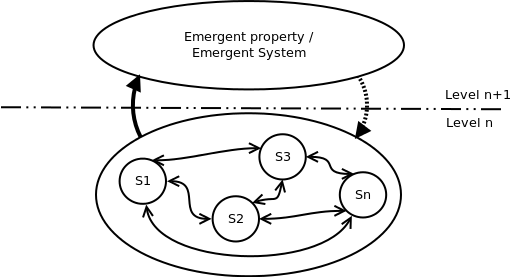
\includegraphics[width=0.9\textwidth]{Emergentism}
  \caption{Modelo de emergentismo}
  \centering
  \label{fig:Emergentism} %\ref{fig:Emergentism}
\end{figure}

En este sentido la auto-organización sucede cuando componentes, sistemas o personas se organizan sin aparente dirección o mando controlador y generan espontáneamente una forma global de orden o coordinación. Esto se da en una gran variedad de fenómenos físicos, químicos, biológicos, sociales y sistemas cognitivos. A nosostros nos incumbe principalmente lo relacionado a lo social e informático. 

\subsection{Sinergia}

En lo social se sabe que se pueden lograr equipos de personas con una alta organización y coordinación sin la necesidad de un líder director, sin un lider que ordene y controle, e incluso sin planificación alguna. Pues, no solo organización y coordinación se puede lograr desde equipos auto-organizados, sino que también se puede lograr sinergia. La sinergia es la prestancia extra que puede dar un equipo debido a la acción conjunta de individuos en equipo que es superior a la suma de las individualidades. Otra propiedad emergente que se puede lograr en grupos auto-organizados es la inteligencia colectiva o inteligencia enjambre que incluye a la "Ley de Linus" y a la "Sabiduría de grupo".

\subsection{Ley de Linus}

Se pueden formar muchos tipos de inteligencia colectiva en equipos colaborativos. Por ejemplo, lo más común en el desarrollo de software es que problemas extremadamente complejos solo pueden ser resuelto por un conjunto de personas trabajando conjuntamente en él, a pesar de que muchas veces sea una sola persona la que resuelva un determinado problema, esa persona nunca podría haberlo hecho sola. Es decir que, dada una base suficiente de desarrolladores y testers validadores colaborando, casi cualquier problema puede ser caracterizado rápidamente, y su solución ser obvia \cite{Eric-Raymond-1997}. A esta idea de inteligencia colectiva se la denomina "Ley de Linus".

\subsection{Sabiduría de multitud}

La Sabiduría de grupo o de multitudes es una idea, apoyada en evidencias, de que dada "ciertas condiciones" las decisiones o predicciones tomadas colectivamente por un grupo de personas suelen ser más atinadas que las decisiones o predicciones individuales o que las que son tomadas sobre la base del conocimiento de un experto \cite{James-Surowiecki-2005}\footnote{"The wisdom of the crowd is the collective opinion of a group of individuals rather than that of a single expert." \cite{MIT-Press-2009}}. Es más, a medida que el grupo es más grande, las decisiones o predicciones son mas acertadas.

Claro que para que esto suceda deben cumplirse ciertas condiciones. Para Surowieki (escritor del libro La Sabiduría de las Multitudes\footnote{\cite{James-Surowiecki-2005}}) las condiciones necesarias son:

\begin{enumerate}

\item \textbf{Diversidad:} el grupo debe tener diversidad de perfiles para lograr una diversidad de Opiniones. Pues, si todos los del grupo piensan igual o semejante, pertenecen a la misma tribu urbana u subcultura, son de la misma profesión o tienen las mismas características de perfil profesional o psicológico, entonces es menos probable de que logren una sabiduría de grupo.

\item \textbf{Independencia:} el grupo no debería estar influenciado y las opiniones de los integrantes tampoco. Si las personas son influenciadas por el grupo se puede caer en lograr el "pensamiento de grupo" y tomar decisiones malas o irracionales. Por otro lado, si el grupo es influenciado por un actor externo al grupo, la decisión grupal es dirigida y, hasta en algún sentido, manipulada.

\item \textbf{Agregación:} El sistema de decisión grupal debe ser agregativo, que significa que debe tener la capacidad de sumar o promediar las opiniones individuales. Un sistema de votación no agregativo, por ejemplo por votación de la mayoria sobre una alternativa, puede hacer prevalicer una decisión individual. Un ejemplo de agregación es cuando la decisión métrica grupal se basa en el promedio de todas la decisiones\footnote{Un ejemplo de Sabiduría de multitud es cuando se le pide a muchas personas que predigan la cantidad de elementos contenidos en un frasco transparente. Es sorprendente como el promedio se acerca considerablemente al número real.}.

% Yo agregaría pericia. 
% Pues si juntamos un montón de filósofos, escritores y médicos a estimar una tarea de desarrollo informático es muy probable que fallen en hacerlo. 

\end{enumerate}

\subsection{Arquitectura emergente}

Hay dos formas extremas de ver el desarrollo de software incluyendo al diseño de software. Una es la que sugiere que se pueden preveer todas las cientos de miles de cuestiones que emergen cuando se desarrolla el software y, en consecuencia, se trata de limitar las respuestas a las mismas conduciendo un desarrollo planificado, estructurado, dirigido y liderado (el extremo izquierdo del aspecto que se muestra en la figura \ref{fig:DesignSpectrum}) \cite{Neal-Ford-2010}. La otra forma es no anticipar nada, permitiendo que las soluciones software emergan espontáneamente a medida que evoluciona el desarrollo en un proceso no dirigido, no liderado y descentralizado (el extremo derecho del aspecto que se muestra en la figura \ref{fig:DesignSpectrum}). En la primera opción el rol de los líderes y expertos (por ejemplo líderes de proyecto y arquitectos expertos), las reglas globales de dirección, el trabajo de comienzo y la información inicial es fundamental para el desarrollo. En el lado de la segunda opción, la orientada a fenómenos emergentes, el rol de todos los actores, el trabajo en equipo y las reglas locales de trabajo son lo principal para el desarrollo. La emergencia de la arquitectura se da, entre otras cosas, cuando se crea una arquitectura inicial simple y flexible, con decisiones tomadas que no son irreversibles, y con una evolución en el tiempo que considera a los nuevos requisitos y problemas que surjan.

\begin{figure}[h] 
  \centering
  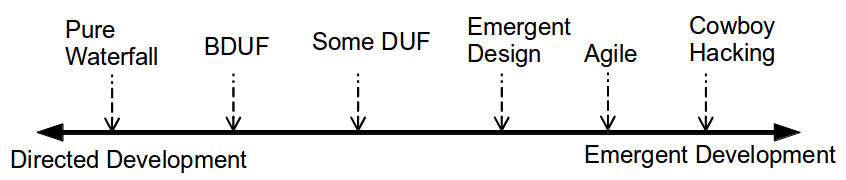
\includegraphics[width=0.99\textwidth]{DesignSpectrum}
  \caption{Modelo del espectro del tipo desarrollo de software}
  (Espectro que abarca el diseño \cite{Neal-Ford-2010})
  \centering
  \label{fig:DesignSpectrum} %\ref{fig:DesignSpectrum}
\end{figure}

Hay una obra literaria llamada "La catedral y el bazar"\footnote{\cite{Eric-Raymond-1997}} escrita por el hacker Eric S. Raymond en 1997 que expone esta idea. La misma analiza dos modelos de producción de software: la catedral que representa el modelo de desarrollo más hermético y vertical (el lado izquierdo de la figura \ref{fig:DesignSpectrum}) y por otro lado el bazar, con su dinámica horizontal y bulliciosa (el lado derecho de la figura \ref{fig:DesignSpectrum}).

\subsection{Resiliencia}

Generalmente no queremos ser frágiles y vulnerables. Y en trabajo de equipos no queremos equipos frágiles trabajando con procesos o marcos vulnerables que ante perturbaciones negativas del medio en dominios complejos tiendan a desmoronarse o producir resultados insatisfactorios. Es conveniente todo lo contrario y se puede caer en pensar que es mejor un equipo robusto. Pero sin embargo, mejor que un equipo rubusto es un equipo resiliente. 

Un aspecto de la filosofía ágil que en muchas ocasiones se hace incapié, aunque generalmente no se explicite, es el de resiliencia. La resiliencia es la propiedad emergente humana que se expresa como habilidad para surgir de la adversidad, adaptarse, recuperarse y acceder a una vida significativa y productiva\footnote{\cite{OPS-OMS-1998}}. Y es justo esa propiedad la que se intenta lograr emerger de equipos ágiles. Los equipos resilientes son aquellos que "asumen las dificultades como una oportunidad para aprender" y "son flexibles ante los cambios" para lograr respuestas positivas y productivas. Bajo esta perspectiva, un equipo consiste en personas que trabajan bajo presión para hacer todo lo mejor que puedan, manejando los conflictos y teniendo recursos para hacer usos de ellos cuando se necesario. Esta no es una propiedad fácil de lograr en los equipos, pero puede condicionarse su emergencia logrando que el equipo trabaje con coraje, compromiso, respeto y apertura basada en relaciones colaborativas y flexibles para tener respuestas positivas ante el cambio. Scrum es el marco de trabajo que permite fallar rápido para aprender de ello y mejorar. Promueve, en su dinámica, el momento de "oportunidad para aprender" y su forma de desarrollo evolutivo permite la "flexibilidad ante los cambios" para no ser frágil, absorviendo las perturbaciones del entorno y transformándolas en algo positivo.

\subsection{Prácticas emergentes}

Scrum se promueve en un dominio de prácticas emergentes. Esto significa que no se puede mecanizar un proceso determinado bajo Scrum para obtener resultados exáctamente predecibles y repetibles en forma estandarizada. Las soluciones no son necesariamente replicables con los mismos resultados, pues sucede que ante los mismos problemas y requerimientos pueden surgir diferentes soluciones. Esto se debe, entre otras cosas, a que las personas no son iguales y los contextos tampoco. Para trabajar bajo Scrum es necesario seguir el núcleo de Scrum, pero implementando diferentes prácticas, técnicas y metodologías, con un grado de experimentación con fallos que intentan ser de bajo impacto. Para lograr una prestancia alta usando Scrum son necesarios niveles altos de creatividad, innovación, interacción y comunicación. En vez de determinar un proceso completo y estructurado, se intenta desarrollar un proceso flexible donde el equipo es quien va generando, sobre la marcha de un proyecto, el proceso propio, de forma tal que el mismo emerge de un contexto relacional e iterativo de inspección y adaptación constante. Son los equipos quienes van encontrando las mejores maneras de resolver los problemas con prácticas emergentes. El conocimiento surge a partir de la acción experimental en prácticas emergentes, rediseñándonos continuamente en busca de una mejor manera, emergente desde lo empírico, de hacer las cosas, sin pretender controlarlas anticipadamente sino, más bien, esculpiéndolas en la práctica constante e iterativa.
       % Principles and values
% Chapter about Scrum System core

\chapter{Núcleo del Sistema Scrum}

Scrum es un sistema compuesto por la filosofía Scrum (SCRUM Philosophy), como parte del sistema cultural, y tres conjuntos de componentes interrelacionados que forman el Núcleo del Sistema Scrum (ver figura \ref{fig:ScrumSystemCore}). Los tres conjuntos de componentes son: roles, actividades y artefactos. Los roles conforman un sistema de roles que determina las responsabilidades de los actores integrantes, sus relaciones recíprocas, sus restricciones y la relación con los demás componentes. Las actividades conforman la parte principal del sistema de procesos Scrum (Proceso Scrum) que determina las relaciones de organización entre actividades, roles y artefactos. Y los artefactos conforman el conjunto de almacenes o componentes de trabajo. Todo el sistema busca asegurar una cadencia de trabajo que consta de una regularidad basada en iteraciones de tiempo fijo y ceremonias o actividades regulares que permiten la repetibilidad rítmica (predictibilidad del flujo de trabajo) bajo un grado de prestancia.

A continuación se describirán estos componentes y sus relaciones.

\begin{figure}[h]
  \centering
  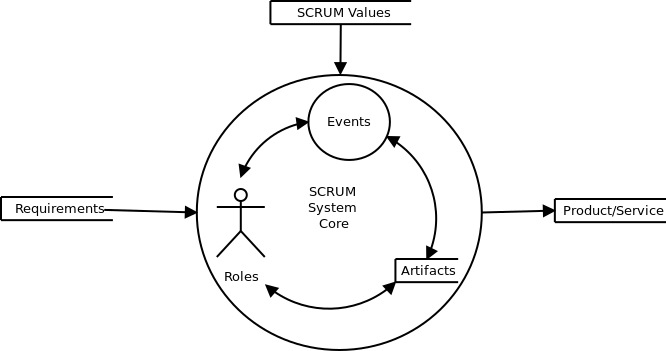
\includegraphics[width=0.99\textwidth]{ScrumSystemCore}
  \caption{Diagrama del Núcleo del Sistema Scrum}
  \centering
  \label{fig:ScrumSystemCore} %\ref{fig:ScrumSystemCore}
\end{figure}


\section{Estructura del Sistema Scrum}

Scrum está pensado como un sistema de trabajo para equipos con tres roles principales: el Product Owner, el Scrum Master y el Development Team. 

Cuando los integrantes del sistema Scrum ejercen los roles mencionados en un flujo de trabajo o proceso Scrum, trabajan sobre tres artefactos esenciales: el Product Backlog (lo que queda por hacer), el Sprint Backlog (lo que se va a hacer) y el Incremento de Producto (lo que logramos hacer). Estos artefactos son tratados en un flujo de trabajo en el cual se construyen productos en forma incremental, en una serie de ciclos cortos de tiempo llamados Sprints. 

En cada ciclo Sprint del flujo de trabajo se practican seis actividades Scrum: refinamiento de producto, planificación, reunión diaria o Daily, desarrollo, revisión de producto y retrospectiva. La actividad de refinamiento de producto (Refinement) no suele tener un nombre unificado; pues, se la suele llamar "Backlog Grooming"\footnote{No se aconseja usar el término Grooming debido a que según el diccionario Oxford English Dictionary tiene connotaciones sexuales.} (aunque no se aconseja usar la palabra grooming), Manteniemiento de Backlog o Refinamiento (Refinement). Salvo el desarrollo, las actividades se consideran reuniones o ceremonias Scrum. El desarrollo no es una reunión Scrum ya que constituye la actividad de producción del producto o servicio. O sea que es donde se produce el incremento de producto.

\section{Sistema de Roles}

El Sistema de Roles (ver figura \ref{fig:ScrumRolesSystem}), en el núcleo de Scrum, es el conjunto de roles y relaciones parte del sistema Scrum. Como se mencionó anteriormente hay tres roles principales: el Product Owner o dueño del producto, el Scrum Master o facilitador y el Equipo de Desarrollo o Equipo a secas (Scrum Development Team, Miembros del Equipo de Desarrollo o Desarrolladores Scrum). También hay roles secundarios como el de Stakeholder, Vendedores y Cuerpo de Asesoramiento de Scrum. El rol Stakeholder es el más importante de los roles secundarios e incluye a los clientes, usuarios y patrocinadores\footnote{\cite{SBOK-2013}}.

Hay que tener en cuenta que Scrum contempla solo estos tres roles principales como núcleo en el equipo Scrum y cuando se implementa en forma ortodoxa son los únicos roles permitidos. En el caso del Equipo de Desarrollo, cada integrante puede tener diferentes perfiles, características o roles especializados, pero bajo este marco sólo tienen el rol de Desarrollador. Cuando Scrum se integra con otras metodologías o esquemas de roles los desarrolladores pueden cumplir otros roles que funcionan como sub-roles.

\begin{figure}[h]
  \centering
  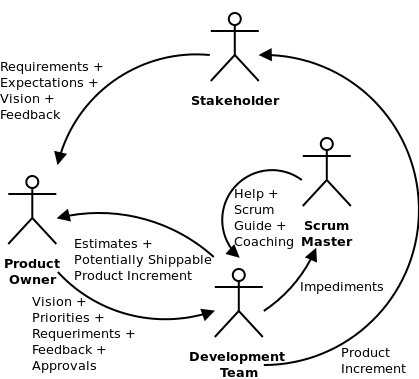
\includegraphics[width=0.80\textwidth]{ScrumRolesSystem}
  \caption{Diagrama del Sistema de Roles Scrum}
  \centering
  \label{fig:ScrumRolesSystem} %\ref{fig:ScrumRolesSystem}
\end{figure}

A continuación se listan los diferentes roles principales:

\subsection{Equipo de Desarrollo}

El Equipo de Desarrollo es parte del Equipo Scrum y son los responsables de construir, o sea desarrollar el producto.
 
Para el cumplimiento del rol Equipo de Desarrollo o desarrollador se deben tener en cuenta las siguientes afirmaciones:

\begin{itemize}
\item Crea y gestiona el desarrollo de software comprometiéndose a fechas de entregas estimadas.
\item Es responsable de la calidad técnica del producto.
\item Debe buscar su desarrollo profesional para lograr excelencia técnica. Para ello debe, además, mantener el foco en el aprendizaje, la innovación y el mantenimiento de una actitud de mejora contínua.
\item Debe evitar trabajar en múltiples proyectos teniendo asignación cien por ciento en el proyecto.
\item Debe priorizar y promover la comunicación cara a cara.
\item Provee estimaciones de ítems de trabajo.
\item Es responsable de gestionar su propio trabajo durante el Sprint.
\item Buscar encontrar una cadencia sostenible para la entrega de incrementos potencialmente entregable de productos.
\item No debe esperar a que le asignen tareas ya que debe seguir la forma "pull" de asignación que consiste en tomar tareas por sí mismo o por consenso de todo el equipo.
\item Monitorea el progreso y el éxito con el resto de los roles del Scrum Team.
\item No debe ocultar impedimentos ni información.
\item No debe hacer tareas de otro rol Scrum. En el caso de una implementación ortodoxa no tiene otro rol que el de desarrollador.
\item Debe procurar ser multidisciplinario aprendiendo del conocimientos de los compañeros, aplicando sus habilidades en diferentes tipos de tareas y no especializándose en una sola cosa donde se trabaja en forma estanco (cerrada y hermética).
\item Debe procurar la estabilidad del equipo y su cadencia.
\end{itemize}

\subsection{Product Owner}

El "Product Owner" cumple la función de dueño del producto en el proyecto y es el responsable del negocio. O sea que, es el "Responsable del Producto" o Servicio, quien vela por que el equipo tenga una visión clara y una estrategia, de qué es lo que se va a hacer, para la creación de ese producto o servicio.

Para el cumplimiento del rol Product Owner se deben tener en cuenta las siguientes afirmaciones:

\begin{itemize}
\item Debe colaborar con el Scrum Master y con el Equipo de Desarrollo.
\item Es quien determina el mejor producto a conseguir.
\item Es quien provee las "hipótesis requerimientos"\footnote{Bajo el marco Scrum los requerimientos inicialmente constan de hipótesis a ser evaluadas. Son hipótesis porque son dinámicas, no son requerimientos finales sino que son deseos del cliente a ser refinados hasta convertirse en verdaderamente requerimientos.}, por lo que es responsable de entenderlas, escribirlas y transmitirlas en forma eficaz.
\item Es dueño y responsable por el artefacto Product Backlog.
\item Es responsable de formar una visión, comunicarla y promoverla.
\item Es responsable del retorno de la inversión ROI y de los resultados empresariales, evaluando continuamente el impacto en el negocio.
\item Es recomendable que esté asignado a un solo Scrum Team con un porcentaje de asignación del 70 al 80 por ciento.
\item Asegura la Colaboración efectiva y la participación de los Stakeholders en el proyecto, administrando sus expectativas y manteniendo una comunicación regular con ellos.
\item Monitorea el progreso y el éxito con el resto de los roles del Scrum Team.
\item No estima ni provee estimaciones.
\item No gestiona el presupuesto de todo el proyecto pero puede gestionar el presupuesto del equipo.
\item No es jefe ni gerente de proyecto.
\end{itemize}

\subsection{Scrum Master}

El Scrum Master es un "Facilitador" y "Coach del Equipo", que es guardián del marco de trabajo Scrum y responsable de mejorar el flujo de valor hacia el cliente. Que sea guardián del marco de trabajo significa que es quien debe asegurar que se siga el sistema Scrum, concientizar sobre la filosofía seguida bajo el mismo, capacitar y entrenar al equipo de desarrollo y facilitar la resolución de impedimentos relacionados a la implementación de Scrum.

Para el cumplimiento del rol Scrum Master se deben tener en cuenta las siguientes afirmaciones:

\begin{itemize}
\item Es el responsable de que se siga Scrum. Brinda apoyo a las prácticas de Scrum.
\item Necesita desempeñar su rol con coraje.
\item Debe gestionar los riesgos y problemas junto con los demás roles.
\item Debe buscar remover obstáculos e impedimentos.
\item Es responsable de buscar lograr la mejora continua del proceso o sistema de trabajo.
\item Busca conseguir que se haga el trabajo.
\item La mejor manera de cumplir el rol es estar tiempo completo en este rol (asignación 100 por ciento).
\item Sirve de embajador del equipo ante la organización, obrando en ocasiones como mensajero, representante o interfaz.
\item Debe ser guardián del equipo protegiéndolo de perturbaciones externas negativas.
\item Monitorea el progreso y el éxito con el resto de los roles del Scrum Team.
\item Ayuda al Equipo a encontrar una cadencia sostenible para la entrega de incrementos potencialmente entregable de productos. 
\item Busca lograr un entorno seguro y de apoyo que genere confianza y respeto mutuo. Ayuda a lidiar con los conflictos personales.
\item Busca establecer acuerdos claros y que se cumpla lo pactado.
\item Colabora con el proceso de aprendizaje del equipo.
\item Considera diferentes formas de trabajar con el equipo Scrum buscando aplicar las más adecuadas según el contexto.
\item Busca comprender la esencia de la comunicación en los diálogos del equipo Scrum y ayudar a concretar sus acciones y su entendimiento.
\item La presencia en la Daily Scrum no es obligatoria, pero es aconsejable que esté para facilitarla y moderarla cuando sea necesario.
\item No debe estimar junto al Equipo de Desarrollo ni hacer tareas de otro rol como, por ejemplo, desarrollar (programar, probar, etc.).
\item No es jefe, no es gerente de proyecto, no debe gestionar al Equipo de Desarrollo y no es responsable por la planificación del proyecto.
\item No asigna tareas, sino que procura que el equipo se las auto-asigne o las tome por voluntad propia y auto-organización.
\end{itemize}


\section{Proceso Scrum}

En el proceso Scrum o sistema de flujo de actividades Scrum (ver figura \ref{fig:ScrumFlow}) los miembros del equipo Scrum colaboran para crear una serie de Incrementos de Producto durante iteraciones de intervalos fijos de tiempo denominados Sprints. En cada iteración Sprint, se comienza por una Planificación del Sprint para producir un Backlog del Sprint a partir del Backlog de Producto, es decir un plan para el Sprint. El equipo se auto-organiza para realizar el Desarrollo, mediante reuniones Diarias de Scrum para coordinar y asegurarse de estar produciendo el mejor Incremento de Producto posible en el proceso de desarrollo del producto o servicio. Cada incremento satisface el criterio de aceptación del Product Owner y la Definición de Hecho o "Definition of Done" compartida por el equipo para satisfacer el criterio de tarea terminada. Junto al proceso de desarrollo se hace también un Refinamiento del Backlog ("Refinement") para prepararse para la reunión de planificación del próximo Sprint. Finalizando cada ciclo se termina el Sprint con una reunión de Revisión del Sprint y luego una reunión Retrospectiva del Sprint, revisando el producto y su proceso con una perspectiva crítica y de mejora contínua. 

\begin{figure}[h]
  \centering
  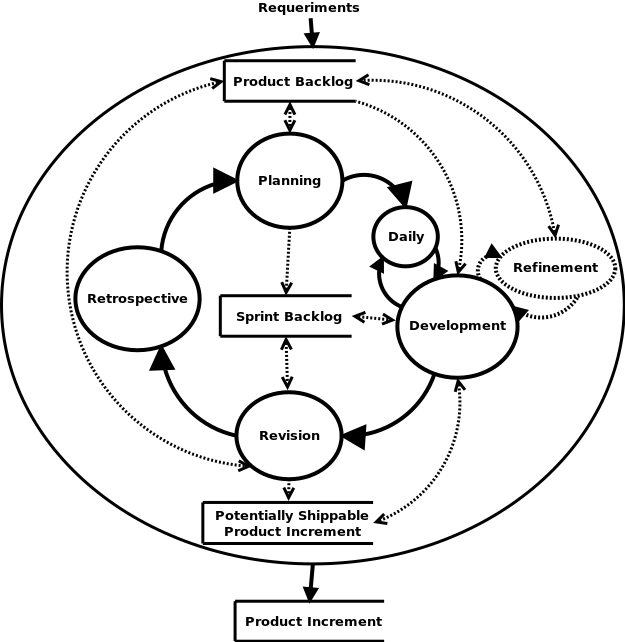
\includegraphics[width=0.99\textwidth]{ScrumFlow}
  \caption{Diagrama de Flujo de Datos del Proceso Scrum}
  \centering
  \label{fig:ScrumFlow} %\ref{fig:ScrumFlow}
\end{figure}

\subsection{Reuniones principales}

\begin{itemize}

\item \textbf{Planificación:} es una actividad o una conversación de duración fija al principio de cada Sprint para decidir sobre lo que se terminará y se demostrará en la revisión.

Esta reunión se divide generalmente en tres partes principales: una primera parte es estratégica relacionada al "qué", una segunda parte táctica relacionada al "cómo" y una tercera relacionada al acuerdo de cierre. 

\begin{itemize}

\item \textbf{Planificación relacionada al "Qué":} La primera parte se propone responder a: ¿Qué trabajo será realizado? En esta parte se desarrolla la definición de lo que se necesita hacer, de cuáles hipótesis del Cliente se desean desarrollar. En este proceso se crean los ítems de Product Backlog o PBIs y los Criterio de Aceptación. Los PBIs son generalmente escritos por el Product Owner y están diseñados para asegurar que las hipótesis de requisitos del Cliente estén claramente representados y puedan ser plenamente comprendidos por todos los Stakeholders y los desarrolladores del Equipo.
En la dinámica de la reunión el Product Owner cuenta cuáles son los PBIs disponibles, que pasan el criterio de completitud o DoR (una definición de terminado), para ser desarrollados en el Sprint y los explica para que sean comprendidos por el Equipo. Mientras sucede esto los integrantes del Equipo hacen todas las preguntas que consideren necesarias para comprender los detalles de lo que se desea realizar y puedan, así, entregar una estimación del trabajo a comprometer. Luego de estimar se procede a una negociación entre el Product Owner y el Equipo de cuáles son los PBIs que el Equipo se compromete a desarrollar para transformar en un incremento de producto potencialmente entregable. En este proceso el Scrum Master se encarga de facilitar la ceremonia, moderar y tratar de asegurar de que todos los Stakeholder del proyecto que sean necesarios para para aclarar detalles estén presentes o sean contactados para hacer las respectivas aclaraciones.
El resultado de este proceso es un conjunto de PBIs estimados y comprometidos inicialmente para ser trabajados en el Sprint.

\item \textbf{Planificación relacionada al "Cómo":} En la segunda parte de la planificación se propone responder a: ¿Cómo será realizado el trabajo? Esta parte es táctica y por lo tanto más técnica por lo que no es necesaria la presencia del Product Owner, pero debe estar disponible para contestar preguntas y clarificar dudas surgidas sobre la marcha. En esta reunión el Equipo discute cómo implementará los PBIs, diseñando inicialmente, en forma general y abstracta (acuerdo de alto nivel), las soluciones y definiendo tareas implicadas. 

\item \textbf{Cierre de planificación como "Acuerdo":} Cuando termina la reunión relacionada al "Cómo", el Equipo debe negociar y comprometer finalmente el alcance del Sprint formando un acuerdo de compromiso con el Product Owner. El resultado de este proceso es un conjunto de PBIs que forman el alcance del Sprint, o sea el Sprint Backlog, el objetivo del Sprint y una visión de diseño o arquitectura a alto nivel de lo que se desea implementar junto con un conjunto de tareas planificadas para el Sprint.

\end{itemize}

\item \textbf{Scrum Diario:} es una actividad o una reunión diaria obligatoria del Equipo Scrum, en el lugar de trabajo, con una duración fija, que sirve para coordinación y organización mediante una retroalimentación del estado de actividades de cada integrante del Equipo. Permite identificar impedimentos bloqueantes, actualizar artefactos, revisar el Sprint Backlog, ayudar a disminuir riesgos e identificar personas que pueden servir de ayuda a determinadas tareas. En esta reunión los miembros del equipo se reúnen, de pie, para informar de sus progresos en el Sprint y planificar las actividades del día. Para ello proporcionan respuestas a tres preguntas:

\begin{itemize}
\item{¿Qué hice ayer?}
\item{¿Qué voy a hacer hoy?}
\item{Si tengo obstáculos: ¿Qué impedimentos tengo?}
\end{itemize}

Es obligatorio que el Equipo asista a esta reunión y es aconsejable que esté el Scrum Master para facilitarla y servir de moderador. El PO puede asistir también para seguir el avance del trabajo durante la iteración, pero puede no participa activamente, sino como oyente. Sin embargo, si se quiere lograr un mejor trabajo de equipo y mayor integración con el PO, es aconsejable que siga la dinámica al igual que el Equipo.

\item \textbf{Refinamiento:} es una actividad o reunión para refinar la lista de PBIs o Product Backlog que consiste en trabajar sobre las hipótesis de requerimientos, definirlas y añadirles detalles, granularizarlas, estimarlas y priorizarlas. Es un proceso continuo que hace el Product Owner, pero formalmente como reunión se desarrolla con participación del Equipo en colaboración para examinar y revisar los elementos del Product Backlog. En esta reunión la responsabilidad recae en el Product Owner y el Equipo solo colabora.

En la reunión que se hace con el equipo se desarrollan las siguientes actividades:
  \begin{itemize}
  \item{El PO presenta los próximos ítems de backlog al equipo.}
  \item{Se conversa grupalmente aspectos sobre ítems de backlog: }
    \begin{itemize}
    \item{Conversación, entendimiento y ajuste.}
    \item{Búsqueda de posibilidad de granularización.}
    \item{Identificación de dependencias.}
    \item{Detección de riesgos que pueden hacer que esas historias no se completen e identificación de actividades a realizar para mitigarlos.}
    \end{itemize}
  \item{Estimación.}
  \item{Priorización.}
  \end{itemize}

\item \textbf{Revisión:} es una actividad o una conversación de duración fija al final de cada Sprint para dar retroalimentación sobre el avance del producto. En esta reunión se evalúa el incremento funcional potencialmente entregable construido por el Equipo en el proceso de desarrollo. Para lograr hacer esto el Equipo de Desarrollo junto al Product Owner y los Stakeholder involucrados, revisan los resultados funcionales y operativos (producto utilizable) del Sprint. El objetivo es recibir una retroalimentación de lo construido y aprobar o rechazar los PBIs que pasaron la DoD y son potencialmente entregables, para lo que los Stakeholder prueban el producto construido y proveen su feedback. En este proceso pueden haber cambios o nuevas hipótesis de requisitos que surjan para agregarse en el Product Backlog.

\item \textbf{Retrospectiva:} es una actividad o una conversación de duración fija al final de cada Sprint para que el Equipo reflexione y busque mejoras procedimentales. En esta reunión se intentan responder tres preguntas relacionadas al "proceso": ¿qué se hizo mal?; ¿qué se hizo bien? y ¿que se puede mejorar?
De esta reunión deberían quedar lecciones aprendidas y un listado de acciones a tomar para mejorar la forma de trabajar. Las acciones a tomar deben ser desarrolladas en el siguiente Sprint y analizadas en la retrospectiva del mismo.

\end{itemize}

\section{Flujo de artefactos}

Los artefactos ítems de trabajo fluyen desde que se definen en el Backlog de Producto hasta que se transforman en incremento de producto. Los ítems de trabajo son items de valor para el cliente que comienzan su nacimiento como ítems de backlog o PBIs del Backlog de Producto. Debido a que el dueño del Backlog de Producto es el Product Owner, es él quien crea los PBIs, ya sea por trabajo individual o con la colaboración del Equipo de Desarrollo. Los PBIs son requerimientos que puede escribirse de diferente manera. Es común escribir los PBIs en forma de Historias de Usuario \cite{Cohn-2004}, pero no es un requisito de Scrum. Estos PBIs son refinados por la actividad de Refinamiento de Backlog hecha por el Product Owner y el Equipo de Desarrollo mientras se practica el desarrollo de un Sprint y son priorizados por el ProductOwner. El la la reunión de planificación "Planning" se toman PBIs que cumplan el criterio de aceptación o "Definition of Ready" (2 "Selection") para ser incluidos en el "Sprint Backlog" y el Equipo de Desarrollo pueda trabajar en ellos en el Sprint. A medida que el Equipo de Desarrollo termina un ítem "Sprint Backlog" cumpliendo el criterio de aceptación "Definition of Done" (3 "increment") se genera un Incremento de Producto candidato potencialmente entregable (Potentially Shippable Product Increment). Luego en la Revisión se acepta el Incremento de Producto candidato pasando a ser efectivamente un Incremento de Producto listo para ser entregado o desplegado, para "Release" (4 "releasing"). En caso de no ser aprobado (5 "Rejection") pasa nuevamente al Product Backlog para ser tenido en cuenta en el próximo Sprint. Los ítems de "Sprint Backlog" que no se lograron terminar también vuelven (6 "comeback") al "Product Backlog". Esto ocurre formalmente en la revisión \cite{Martin-Alaimo-2014}.

\begin{figure}[h]
  \centering
  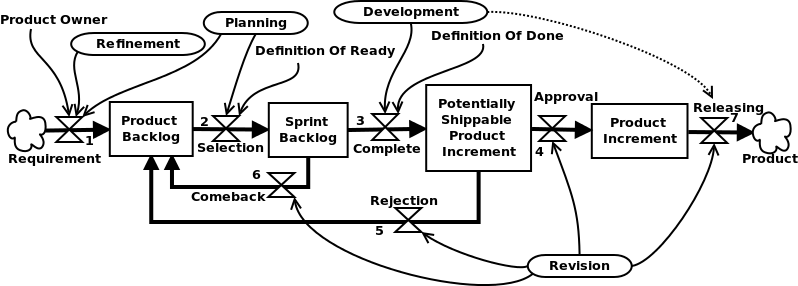
\includegraphics[width=0.99\textwidth]{ScrumArtifactsStockFlow}
  \caption{Diagrama de Flujo de Stock de artefactos Scrum}
  \centering
  \label{fig:ScrumArtifactsStockFlow} %\ref{fig:ScrumArtifactsStockFlow}
\end{figure}

\subsection{Definición de preparado}

La definición de preparado, "Definition of Ready" o DoR es una Definición de Terminado particular que se corresponde con las condiciones para que un PBI pueda pasar a formar parte de un Sprint Backlog. Si un PBI no cumple con su DoR no puede ser tomado en una planificación para ser ítem de trabajo del Sprint planeado, ya que es un ítem que no está suficientemente preparado para ser comprometido. O sea que, la definición de preparado permite entonces tener un punto de acuerdo entre el Product Owner y el Equipo, permitiendo conocer cuándo una historia de usuario está realmente lista para evaluar su factibilidad de desarrollo en una reunión de planeamiento y ser llevada a un Sprint.

Un ejemplo de DoR puede ser el que sigue:

\begin{enumerate}
\item{Historia de usuario definida.}
\item{Cumple el criterio INVEST (INVEST es tratado posteriormente).}
\item{Hay un contexto de negocio claro.}
\item{Criterios de aceptación definidos, claros y comprobables.}
\item{Identificación de dependencias con otras historias de usuario.}
\item{Hay una idea clara de cómo se puede demostrar la historia en una review.}
\item{El equipo tiene el conocimiento para analizarla.}
\end{enumerate}

\subsection{Definición de Terminado}

Los ítems de artefactos fluyen por sus diferentes estados (o Stock en el flujo de Stock) a medida que cumplen con determinadas condiciones de cambio de estado. A estas condiciones que deben cumplir para cambiar de estado se las llama definición de terminado y funcionan como válvulas para que los ítems pasen de un Stock a otro Stock. Por ejemplo para que un ítem pase del Stock de Sprint Backlog a Incremento de Producto Potencialmente Entregable debe cumplir una definición de terminado, "Definition of Done" o DoD. Normalmente se suele considerar que el DoD es una lista de actividades que cada elemento de trabajo debe completar para poder ser considerado potencialmente entregable para un cliente dado y conforma un "entendimiento compartido de lo que significa que el trabajo esté completado"\footnote{\cite{Ken-Jeff-2013}}.

\section{Reglas y Consideraciones}

Además se establecen alguna consideraciones relacionadas a tiempos y tamaños. Se aconseja un tamaño de equipo de desarrollo mayor a 4 miembros y menor a diez (7 +- 2), o sea entre cinco y nueve. Por debajo de este número mínimo se tiene un equipo pobre que puede brindar un producto pobre y por sobre ese número máximo se aumenta la complejidad de gestión y coordinación del equipo disminuyendo el funcionamiento apropiado tras la metodología planteada. También se recomienda una duración de Sprint no mayor a un mes \cite{Ken-Jeff-2013}. La Reunión de Planificación de Sprint debería tener un máximo de duración de ocho horas para un Sprint de un mes. El Scrum Diario o "daily" es una reunión con un bloque de tiempo de 15 minutos para que el Equipo de Desarrollo sincronice sus actividades y cree un plan para el día. Por ejemplo, una daily de mayor de 15 minutos se puede considerar larga y en 15 minutos es complicado que mas de 15 personas puedan exponer lo que hicieron, lo que harán y si tienen bloqueos. Por eso se aconseja como máximo nueve personas en el equiopo de desarrollo. En lo que concierne a la Revisión, el tiempo estipulado es de cuatro horas para Sprints de un mes o dos horas para uno de una quincena. La reunión de Retrospectiva  debería estar restringida a un bloque de tiempo de tres horas para Sprints de un mes o  a una hora y media para los de una quincena. Las reuniones de Planificación, Revisión y Retrospectiva deberían ser proporcionales a la duración del Sprint.
     % Process and methodology
\chapter{Gestión de Proyectos}

Scrum es un marco de gestión de proyectos para el desarrollo incremental de productos, valiéndose de equipos autoorganizados. 



\subsection{Proyecto Scrum}

Un proyecto, en ingeniería de software, es un esfuerzo temporal que se lleva a cabo para crear un sistema, software o resultado único\footnote{Se parafrasea la definición del PMBOOK \cite{PMBOK-2004}.}. Los proyectos son organizados, en una empresa u organización, por el proceso de administración de proyectos. Según este proceso, el ciclo de vida de los proyectos se puede dividir en tres fases: inicio, ejecución y cierre (ver figura \ref{fig:PMIProject}). En la administración de proyectos es necesario planificar los proyectos y dicha actividad se suele hacer en la fase de inicio ("Starting phase" o "Project Start"). Pero, a diferencia de la metodología clásica (ver figura \ref{fig:PMIProject}) en que la planificación estaba siempre al inicio y el desarrollo en la fase de ejecución, en el marco Scrum la planificación se distribuye durante todo el ciclo de vida del proyecto y en la fase de ejecución se hace el desarrollo incremental de productos (por incrementos de producto) en iteraciones cortas (Sprint) donde cada iteración tiene su respectiva planificación (ver figura \ref{fig:ScrumProject}) y su incremento de producto, en caso de haberlo logrado.

\begin{figure}[h]
  \centering
  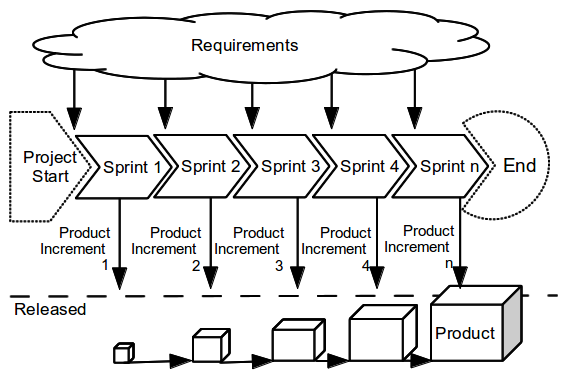
\includegraphics[width=0.90\textwidth]{ScrumProject}
  \caption{Proyecto Scrum}
  \centering
  \label{fig:ScrumProject} %\ref{fig:ScrumProject}
\end{figure}

Entonces podemos decir que en Scrum se piensa en muchos planes periódicos (a corto plazo). Los mismo pueden estar en un plan mayor a largo plazo pero de carácter flexible. También se puede realizar un plan global de entregables en base a los incrementos de producto estimado. Pero, desde esta perspectiva, hay que considerar que aunque se trabaje con planificaciones, los planes no son contratos a respetar a rajatabla.

%Triangle of Project Management
\subsection{Triángulo de la Gestión de proyectos}

El marco de Scrum cambia el triángulo clásico de la gestión de proyectos. El compromiso ya no es entre el tiempo, presupuesto y calidad; sino que se basa en el triángulo de: Presupuesto (Costo), Tiempo y funcionalidad (alcance) (ver figura \ref{fig:ScrumProjectManagementTriangle}). Además, tradicionalmente se ha intentado fijar el alcance para negociar y variar el presupuesto y el tiempo. En cambio, desde la agilidad, se intenta mantener fijos el tiempo y el presupuesto mientras se varía el alcance \cite{Martin-Alaimo-2014}.

\begin{figure}[h]
  \centering
  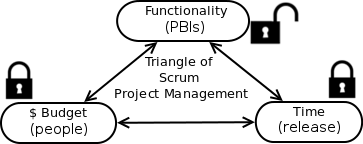
\includegraphics[width=0.80\textwidth]{ScrumProjectManagementTriangle}
  \caption{Triángulo de Gestión de Proyectos Scrum}
  \centering
  \label{fig:ScrumProjectManagementTriangle} %\ref{fig:ScrumProjectManagementTriangle}
\end{figure}

\subsection{Planificación de entregables}

Con esta metodología tampoco es necesario hacer una entrega final (o "releasing") ya que se pueden hacer entregas paulatinas. Para hacer entregas intermedias se puede crear un plan de muy alto nivel para múltiples Sprints durante una planificación de lanzamiento. Este plan de entregables o de de lanzamientos es una guía con la que se pretende reflejar las expectativas sobre las qué funciones se implementarán y cuando se completarán \cite{Scrum-Institute-2015}. También sirve como una base para monitorear el progreso dentro del proyecto. Pero siempre hay que considerar que no es un plan equivalente a un plan clásico, los ítos de releases no deberían ser compromisos rígidos y contractuales, y el desarrollo del proyecto no debería centrarse en respetar el plan. Por este motivo el plan de lanzamiento no es un plan estático. Pues, se cambia durante todo el proyecto cuando nuevos requerimientos o conocimientos están disponible y, por ejemplo, cuando entradas en el Scrum Product Backlog cambian y re-estiman. Por lo tanto este plan debe ser revisado y actualizado en intervalos regulares, por ejemplo, después de cada Sprint.

Para crear un plan de entregables se deben tener disponibles las siguientes cosas:

\begin{enumerate}
\item Un Product Backlog priorizado y estimado.
\item La velocidad estimada del Equipo Scrum.
\item Las condiciones de satisfacción (metas para la agenda, el alcance, los recursos)
\end{enumerate}

\subsection{Métricas}

Las métricas son indicadores que ayudan al equipo a medir su propio desempeño para poder hacer cambios basados en hechos. También es un soporte a la gestión de proyectos para poder medir el avance del proyecto, revisar la productividad y el desempeño\footnote{Las métricas se pueden usar para medir desempeño, pero no se deben utilizar en forma punitiva ni tampoco en sistemas de evaluacion de desempeño de empleados.} del equipo y poder hacer comparaciones entre evolución de diferentes equipos. 

\subsubsection{Unidades de medida}

Para poder usar métricas y medir es necesario unidades de medida. Las más usadas son:

\begin{enumerate}

\item {\textbf{Story Points:}
El Story Points o SP es una unidad de medida que indica una cantidad de alcanse o trabajo que puede ser entregado o tamaño de producto estimado para entregar. Es una unidad de medida que representa la complejidad o esfuerzo necesario para terminar las tareas de una historia \footnote{\cite{Jipson-Thomas-2015}}. El SP sirve como estimación de la complejidad en forma relativa y sumativa que hacen los desarrolladores. También hay que tener en cuenta que es una unidad subjetiva que depende de qué equipo hace la estimación de medida.
}

\item {\textbf{Business Value Point:}
El Business Value o BV es el valor añadido que la historia aporta al negocio\footnote{\cite{Pointet-Botton-2012}}. A semejanza del SP, el Business Value Point o BVP sirve como estimación del valor de negocio en forma relativa y sumativa que hace el PO. También hay que tener en cuenta que es una unidad subjetiva que depende de qué PO o equipo de personas hace la estimación de medida.
}

\end{enumerate}

\subsubsection{Mediciones}

Hay muchas mediciones que nos pueden ser de utilidad, como por ejemplo las siguientes\footnote{Scott y Jeff \cite{Scott-Jeff-2013} y la  Scrumalliance en un artículo llamado "Velocity, How to Calculate and Use Velocity to Help Your Team and Your Projects", por Catia Oliveira (6 February 2014).}:

\begin{enumerate}

\item {\textbf{Velocity:} La 'velocidad'\footnote{"Sum of original estimates of all accepted work" \cite{Scott-Jeff-2013}.} es el número de unidades de trabajo o puntos de historia SP estimados y aceptados por un equipo en una iteración Sprint. En otras palabras, es el conjunto de puntos de historia totales conseguidos por el equipo al final de cada Sprint\footnote{\cite{Jipson-Thomas-2015}}.}

Esta definición es la clásica y es algo genérica. Hay tres formas más específicas de interpretar y medir la velocidad:

  \begin{enumerate}

  \item{\textbf{Velocidad de trabajo:} cuando la velocidad muestra la cantidad de trabajo o funcionalidad que un equipo entrega (aceptada) en un sprint\footnote{\cite{SBOK-2013}}, incluyendo las de valor indirecto. En este sentido las historia de usuario completadas (tomadas del backlog técnico) que tienen valor indirecto para el cliente, las correcciones de errores, deuda técnica, migraciones y refactorizaciones sí cuentan en la velocidad. En este caso, la velocidad del equipo da pocas indicaciones sobre el verdadero valor de negocio entregado y más sobre la capacidad que puede producir. Pues la velocidad, en este sentido, no suele tener relación directa con el valor de negocio entregado. Como no se suele aclarar bien la definición de velocidad se suele entender que se trata de esta perspectiva pero, sin embargo, en Scrum clásico se sobreentiende que los equipos deben entregar valor de punta a punta, por lo que la velocidad debería estar ligada al valor como la siguiente definición.
  }

  \item{\textbf{Velocity en nueva funcionalidad:} cuando la velocidad muestra solo la cantidad de funcionalidad de valor para el negocio que un equipo entrega (aceptada) en un sprint. En este sentido las historia de usuario que no tienen ningún valor para el cliente o incompletas, las correcciones de errores y las refactorizaciones no cuentan en la velocidad\footnote{\cite{David-Koontz-2014}}. En este caso, la velocidad del equipo da un indicio sobre el valor de negocio entregado por el equipo. En Scrum original o clásico se sobreentiende que las historias son las que aportan valor, por tal motivo a veces no se aclara explícitamente esto.
  }
  
  \item{\textbf{Value Velocity:} es una forma interesante para medir la productividad (sugerida por James Shore\footnote{\cite{James-Shore-2015}}) similar a la velocidad tradicional o velocidad de trabajo, excepto que se basa en estimaciones de valor de negocio (Business Value Point) hechas por el PO antes de la planeación.
  }
  
  \end{enumerate}

\item {\textbf{Average Velocity:} De la valocity de cada Sprint se calcula la velocidad promedio o "Average Velocity" que es el número de unidades de trabajo o SP promedio estimados y aceptados por un equipo en un conjunto de iteraciones Sprint. En un equipo ágil de velocidad estable, la velocidad promedio (por ejemplo de los últimos 4 Sprints) es un indicador adelantado de la velocidad estimada para el próximo Sprint (bajo las mismas condiciones de los Sprints usados para calcularla).}

\item {\textbf{Work Capacity:} La Capacidad es la suma de todos los trabajos reportados durante el Sprint, esten terminados o no\footnote{Scott y Jeff \cite{Scott-Jeff-2013}}. La capacidad es generalmente igual o superior a la Velocity. Aunque la Capacida puede, en raras ocasiones, caer por debajo de la velocidad. Esto se debe a que la velocidad se calcula en base a las estimaciones originales de trabajo, mientras que la capacidad se calcula en base a la suma de trabajo real reportado\footnote{Scott y Jeff \cite{Scott-Jeff-2013}}. Por lo que en el caso de que esto suceda, lo que indica es que el equipo ha sobre estimando la complejidad de los trabajos solicitados. También existen otras formas de calcular o entender la capacidad. Por ejemplo:

  \begin{enumerate}
  
  \item {\textbf{Capacidad en puntos ideales:} La capacidad puede ser una idealización basada en la velocidad promedio, o sea, los puntos de la historia que se pueden considerar gastar en la próxima carrera de velocidad.\footnote{\cite{Satish-Thatte-2013}}}

  \item {\textbf{Capacidad en horas:} La capacidad puede ser calculada en horas basados en la cantidad de miembros y la cantidad de horas efectivas de trabajo en un Sprint. Por ejemplo en un equipo de 8 miembros, con 6 horas de trabajo efectivo y un Sprint de 10 días, la capacidad en horas es igual a 480 hs (8 x 6 hs x 10).}

  \end{enumerate}

Cuando se definió el marco de trabajo, como algo mínimo de cosas para que funcione, se dejó lo más simple posible. Debido a ello, el concepto de Velocity sí es partes del marco de trabajo, pero Working capacity no lo es, aunque es ampliamente usado \footnote{Erich Buhler, Agilib.org 2015, Proyecto Mercury 2015 (LAN), \cite{Erich-Buhler-Coach-2015}.}.
}

\item {\textbf{Focus Factor:} El Focus Factor es la relación entre la Velocity y la capacidad de trabajo: ( Velocity / Work Capacity ) x 100\%. La misma debe permanecer en la vecindad de 80 \% en promedio para un equipo saludable. Estos puntos de datos por debajo del 80 por ciento indican un equipo que está interrumpido o incapaz de convertir su trabajo estimado en trabajo aceptado mostrando poca previcibilidad. Cuando el valor es alto, cercano al 100, el equipo ha estado bajo la previsión de su capacidad, aunque esto no indica necesariamente que están trabajando bien. Por ejemplo, el equipo puede estar aparentando ser perfecto forzando la coincidencia.}

\item {\textbf{Targeted Value Increase (TVI+)} El TVI+ responde a cuánto cambio ha habido en la velocidad del equipo a través del tiempo desde el primer Sprint. Es la Velocity del Sprint actual dividido la Velocity Original (velocity del primer sprint): ( Current Sprint’s Velocity / Original Velocity ) x 100\%. Sirve para medir el aumento de la contribución de valor de un equipo en base a su velocidad origen Sprint a Sprint.
Por ejemplo, si el resultado es 200\% significa que el equipo ha duplicado su capacidad de resolver con éxito la complejidad requerida.
}

%Otras: Percentage of Adopted Work, Percentage of Found Work, Accuracy of Estimation, Accuracy of Forecast, Targeted Value Increase (TVI+), Success at Scale

\item {\textbf{Business Value Delivered:}
Un indicador relevante es el valor de negocio entregado. Se pueden contabilizar los BV entregados en cada Sprint.
}

\item {\textbf{Happiness Metric:}
Un estudio de Harvard muestra que la felicidad aumenta la producción de cualquier tipo de trabajo, pues "la gente feliz es 12 \% más productiva"\footnote{\cite{U-K-University-2014}}. En base a esto podemos intentar medir la felicidad Sprint a Sprint\footnote{\cite{Jeff-2014}}. 

La felicidad del equipo es un indicativo de la salud del equipo en relación a su capacidad de entrega de valor. Para medir la felicidad del equipo podemos hacer encuestas o responder las siguientes preguntas:

  \begin{enumerate}
  \item {¿Cómo me siento acerca de mi trabajo? Se puede usar una escala de 1 a 5. Otra escala para medir felicidad puede ser de siete puntos. Por ejemplo a la pregunta... ¿Cómo calificaría su felicidad en este momento? Se puede responder con 1 que es totalmente triste, 2 es muy triste , 3 es triste, 4 es ni feliz ni triste, 5 es bastante feliz, 6 es muy feliz y 7 es completamente feliz\footnote{\cite{U-K-University-2014}}.
  }
  
  \item {¿Qué va a hacer que me sienta mejor?}
  \end{enumerate}

Cuando tenemos la información de cada miembro del equipo, el equipo puede hacer una lluvia de ideas de cómo hacer para mejorar y aumentar la felicidad en el siguiente Sprint y darle curso y seguimiento a las acciones propuestas.

También se puede medir la felicidad de los Stakeholder como indicador de grado de satisfacción que indica qué tan contentos estuvieron con los resultados del Sprint y con la Review. Este relevamiento relacionado a la persepción de valor entregado se puede hacer en la misma Review.

}


\end{enumerate}
       % Project Management
\chapter{Escalamiento}

Scrum es aconsejable para ser óptimo en equipos chicos y proyectos pequeños, con agrupación de personas de múltiples disciplinas en un solo equipo para maximizar el ancho de banda de las comunicaciones, la visibilidad y la confianza. Esto sucede porque cuando los equipos son grandes aumenta el acoplamiento de individuos complejizando las comunicaciones y dificultando la coordinación y el buen desarrollo de las reuniones Scrum. Además se desprende del principio o Ley de Brooks, que dice que cuando se agregan personas a un proyecto o equipo aumentan los canales de comunicación pudiendo generar sobrecarga de comunicación. Por este motivo y desde un punto de vista purista, cuando se quiere implementar Scrum en proyectos grandes que requieren muchas personas, en su forma ortodoxa, no es recomendable. Pero se han encontrado maneras organizativas para aplicar Scrum en estos casos, como así también en grandes organizaciones. A esto se llama "Scaling Scrum" o Escalamiento de Scrum.

En "Scaling Scrum" los desafíos más importantes son: manejar las dependencias e integrar el trabajo en todos los niveles. En general Scrum se escala mediante reproducción de equipos con configuraciones adecuadas y la cohesión y acoplamiento mediante algún sistema de integración ágil, como el uso de "Scrum de Scrum", equipos de Product Owners, equipo de integración, etcétera. Hay varios casos que se pueden investigar, como por ejemplo las implementaciones de: Google, Spotify, Adobe, Nexus, etc.

\section{Formación de equipos}

Cuando migramos desde una organización tradicional, de management 1.0, a una ágil, tal vez uno de los desafíos más relevantes y difíciles es el de organizar equipos. ¿Cómo juntamos a las personas apropiadas en forma sostenida en el tiempo? Para que un equipo sea uno, debe tener un propósito claro y distinguible de otro de la compañía. Y, en consecuencia, debería tener todas las habilidades y competencias necesarias para cumplir el propósito de forma sostenida en el tiempo. Cuando ya tenemos equipos Scrum formados, tal vez la tarea sea más fácil. Pues, en "Scaling Scrum" los equipos funcionan como células que, a medida que la organización se expande, se clonan sus estructuras como en reproducción celular. Las estructuras de las células dependen del problema que se quiere resolver en cada caso y según los nuevos propósitos que surjan. 

De esta idea se desprende la pregunta de ¿qué propósito damos a cada equipo? o ¿cómo estructuramos a los equipos según qué propósitos? Una manera de hacerlo, pensando en productos y en el sector de producción de la compañía, es tomando una unidad de negocio o producto y ver si su alcance o tamaño es suficiente para un equipo o para varios. Si es para varios, una forma es analizar la jornada o flujo de experiencia del producto, determinar los KPIs involucrados y desglosar en subproductos con sus KPIs asociados. Así cada equipo puede ser responsable de un subproducto y de impactar según los KPIs identificados. Esta es una manera de hacerlo de arriba hacia abajo y orientados a producto. Luego, otra pregunta que surge es: ¿cómo los estructuramos? Bien, si el equipo es de producción como el desarrollo de software de productos, con trabajo planificable y divisible en lotes, Scrum viene como anillo al dedo. O sea que necesitamos a un SM y un PO en el equipo. Un equipo Scrum puede estar formado por diferentes roles, tales como: UX, SM, PO, BA, QA, FE Dev, BE Dev, etcétera. Por ejemplo, un equipo puede estar formado por: PO, SM, UX, 3 FE Dev y 3 BE Dev; otra estructura puede ser: PO, SM, BA, QA, 2 FE Dev y 2 BE Dev. O sea que podemos tener una infinidad de configuraciones. ¿Cuál puede ser la apropiada? No solo depende del propósito, sino de cómo desarrollaremos ese propósito o cuán autónomos somos en relación a él. En esta vía tenemos tres lineamientos básicos de configuración: equipos Scrum de características, equipos Scrum de componentes o uno mixto. Y cada una de estas modalidades pueden tener diversas configuraciones de roles.

\subsection{Equipos de características}

Abordar el problema de proyectos grandes con "Equipos Scrum de características" consiste en la conformación de equipos totalmente multi-funcionales con un enfoque "Whole Team"\footnote{En un enfoque Whole Team todos pueden hacer, hasta cierta medida, alguna tarea de otro\cite{Juan-Gabardini-2015}.} con características de miembros full-stack, capaces de operar en todos los niveles de la arquitectura del producto con el fin de ofrecer las características centradas en el cliente (ver figura \ref{fig:ScrumTeamsByFeatures}). O sea que cada equipo trabaja sobre determinadas características de producto (Features) o PBIs desarrollando todos los niveles del sistema a desarrollar (end-to-end). En este sentidos, los equipos son homogéneos entre sí pero heterogéneos internamente, con integrantes de habilidades diversas y características profesionales multidisciplinares. Para lograr esto se debe conformar una organización de aprendizaje donde los equipos practican el aprendizaje continuo, donde aprenden para abarcar los componentes arquitectónicos.

\begin{figure}[h]
  \centering
  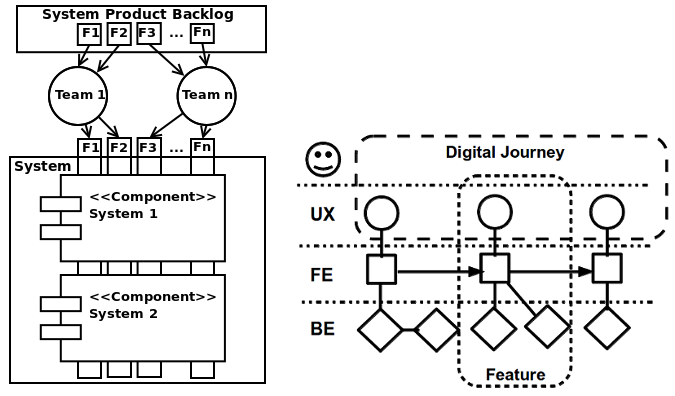
\includegraphics[width=0.80\textwidth]{ScrumTeamsByFeatures}
  \caption{Esquema de equipos de características}
  \centering
  \label{fig:ScrumTeamsByFeatures} %\ref{fig:ScrumTeamsByFeatures}
\end{figure}

En esta arquitectura de organización es necesario coordinar el trabajo de los diferentes equipos. Los Scrum Master deben reunirse con regularidad, promoviendo la transformación a través de una lista visible de los impedimentos de organización. Los Scrum Master, además deberán estar familiarizados con biografía relacionada a este problema de escalabilidad como "Scaling Lean and Agile Development" \cite{Larman-Vodde-2008}.

\subsection{Equipos de componentes}

Abordar el problema de proyectos grandes con "Equipos Scrum de componentes" (ver figura \ref{fig:ScrumTeamsByComponent}) consiste en que cada equipo sólo es responsable de la ejecución de ciertos componentes dedicados en el sistema de los cuales el equipo es dueño de su desarrollo. Desde esta perspectiva se pueden tener equipos dedicados por capas (capa front-end, capa de servicios, capa de persistencia) y por componentes de arquitectura de software (diferentes componentes como librerías, servicios o subsistemas).

\begin{figure}[h]
  \centering
  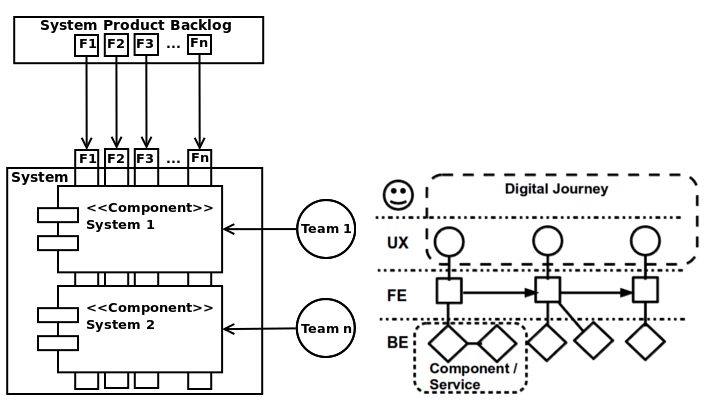
\includegraphics[width=0.80\textwidth]{ScrumTeamsByComponent}
  \caption{Esquema de equipos de componentes}
  \centering
  \label{fig:ScrumTeamsByComponent} %\ref{fig:ScrumTeamsByComponent}
\end{figure}

Para terminar una PBI o historia de usuario hay en la mayoría de los casos la necesidad de dividir las historias en partes más pequeñas que podrían ser implementadas dentro de un solo componente. Además se genera dependencias entre los diferentes equipos haciendo necesario procesos de integración periódica y coordinación de equipos. En muchos casos, una sola historia de usuario no se puede implementar dentro de un único sprint y, en su defecto, depende de los resultados de otras historias desarrolladas por otro equipo que aún no están disponibles. A esto se lo llama "pipeline" y debe evitarse en lo posible o gestionarse apropiadamente.

La ventaja de utilizar equipos de componentes es que es más fácil asegurar una determinada arquitectura del sistema. Por ejemplo si se quiere asegurar una Arquitectura SOA o una de Microservicios que está orientada a componentes. Esta idea está, entre otras cosas, basada en la "Ley de Conway"\footnote{Conway's Law \cite{Conway-1968} no es exactamente una ley, sino que es más bien una observación que Conway publicó en 1968.} que sugiere que las organizaciones pueden replicar su arquitectura en los productos que ellas producen \cite{Martin-Fowler-2014}. 

Por otro lado, puede tener como desventaja que las personas se pueden especializar sólo en pequeñas partes del sistema y el conocimiento global sobre el sistema en su conjunto podría perderse \cite{Scrum-Institute-2015}. En este caso podría tener lugar una optimización local, ya que el equipo a veces puede tomar decisiones que están optimizadas para el componente individual, pero las mejores soluciones desde una perspectiva del sistema total podrían haber sido desestimadas u obviadas.


\subsection{Equipos mixtos}

También es posible la configuración de equipos mixtos que son la combinación de equipos de características y de componentes (ver figura \ref{fig:ScrumTeamsMix}).

\begin{figure}[h]
  \centering
  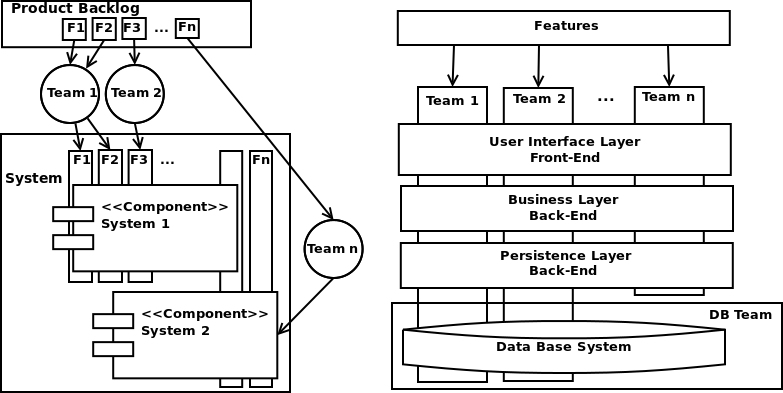
\includegraphics[width=0.99\textwidth]{ScrumTeamsMix}
  \caption{Ejemplo de equipos mixtos.}
  \centering
  \label{fig:ScrumTeamsMix} %\ref{fig:ScrumTeamsMix}
\end{figure}

\section{Integración}

\subsection{Scrum de Scrum}

Scrum de Scrum es una forma de organización y técnica para escalar Scrum a grupos grandes de personas u organizaciones con proyectos grandes, programas o portfolios. Consiste en distinguir un integrante con el rol de Embajador, denominado "Ambassador", por cada Equipo Scrum \cite{Stefanini-2013}. El Embajador será quien participará en reuniones Daily con Embajadores de otros equipos. A esta reunión de Embajadores se la llama "Scrum de Scrum" o SoS. Habitualmente se usa que el rol de Embajador lo desempeñe el Scrum Master, pero puede ser desempeñado por otro integrante del Equipo de Desarrollo. También puede ser desempeñado por un integrante del Equipo acompañado del Scrum Master.

La reunión SoS se comporta como una Daily donde los Embajadores reportan la situación de su equipo y sus impedimentos. El embajador de cada equipo comenta la respuesta a las siguientes tres preguntas:

\begin{itemize}
\item \textbf{¿Qué hicimos ayer?}
\item \textbf{¿Qué vamos a hacer hoy?}
\item \textbf{Si tenemos obstáculos: ¿Qué impedimentos tenemos?} ¿Qué impedimentos tenemos a nivel de equipo? ¿Si algún otro equipo nos bloquea para algo? ¿Si bloqueamos en algo a algún otro equipo?
\end{itemize}

La SoS puede ser facilitada y moderada por una persona que puede desempeñar un rol de facilitador, coordinador e integrador inter-equipos. Este rol puede tener diferentes nombres y el SBOK lo denomina Chief Scrum Master o CSM. El CSM apoyará y brindará soporte a los SM de diferentes equipos.

\subsection{Scrum de Scrum de Scrum}

En organizaciones donde hay muchos Equipo Scrums trabajando en varias partes de un proyecto o producto grande, puede ser necesario otro nivel más de coordinación, ya que hay equipos que no participan en SoS de otras áreas. Aquí es cuando se aplica la "Scrum of Scrum of Scrum"\footnote{\cite{SBOK-2013}} o SoSoS, que consiste en una reunión frecuente a un nivel superior de la SoS.

\subsection{Comunidades}

En una organización grande, independientemente de Scrum, se suelen formar comunidades. Estas comunidades se dan por especialidades técnicas o roles. Las mismas son útiles para colaboración entre equipos, generación de discusiones globales y resolución de problemas transversales. Es aconsejable que se den en forma orgánica. Aunque son particularmente útiles las comunidades de SM y de PO. La de SM es una posibilidad de mejora contínua del marco de trabajo y la de PO puede funcionar como equipos de PO para tratar temas del negocio transversal y administrar backlog en conjunto.

\begin{figure}[h]
  \centering
  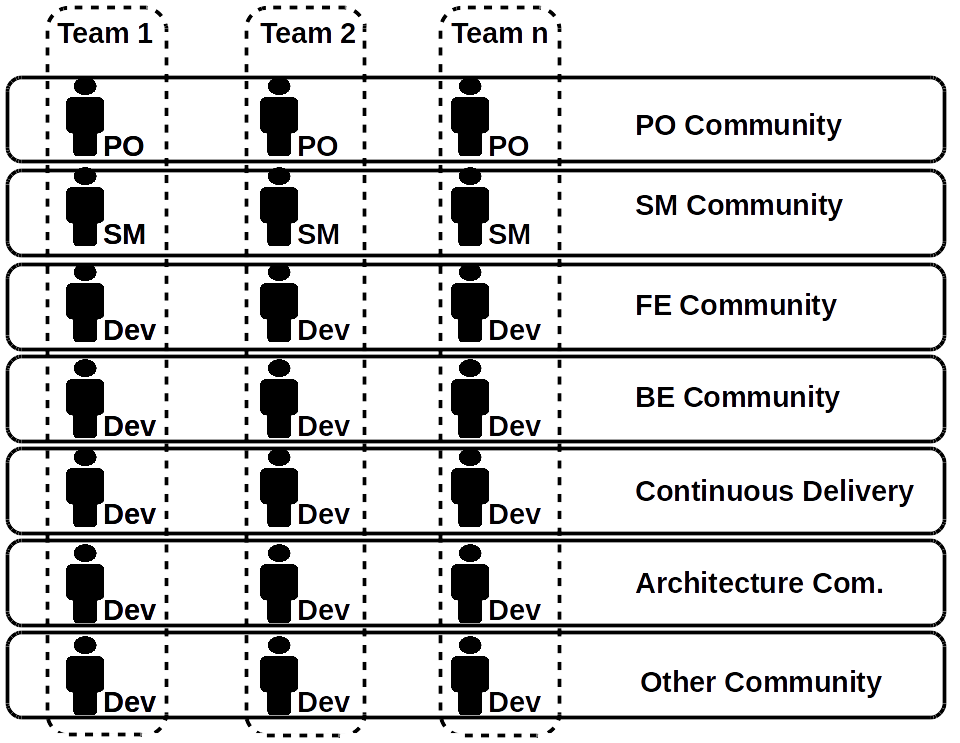
\includegraphics[width=0.60\textwidth]{Communities}
  \caption{Ejemplo de comunidades}
  \centering
  \label{fig:Communities} %\ref{fig:Communities}
\end{figure}


\subsection{Integración UX}

Un desafío a la hora de hacer Scrum es incorporar UX en el desarrollo incremental por sprints. Se pueden adoptar, entre otras, dos estrategias principales: desarrollo UX distribuido y gobernado; o desarrollo UX centralizado (equipo externo).

\subsubsection{Desarrollo UX Distribuido y Gobernado}

Una estrategia es tener UXer, como miembros de equipo Scrum, distribuidos en cada equipo. Esto permite empoderamiento y velocidad, pero puede generar una UX poco unificada o con poca “integridad conceptual”. Para resolver este problema de unificación se puede acudir a la estandarización UX. La misma podría ser generada y mantenida por los equipos o mediante un equipo externo responsabilizado de la integridad conceptual y experiencia unificada (equipo de estandarización UX transversal) y usar un sistema de versionado de estándares que sirve como otra herramienta de coordinación.

\subsubsection{Desarrollo UX Centralizado}

Otra estrategia es tener un equipo externo de UX que agrupe a todos los UXer y que provea, como un equipo de servicios, los diseños UX a los equipos de desarrollo. Sin embargo, es probable que el equipo central se convierta en un “cuello de botella” para los equipos de desarrollo y, además, pueda generar más “dependencias” que deben ser abordadas. Para mitigar estos problemas, un modelo híbrido a menudo puede ser aplicado, además de mecanismos de coordinación entre el equipo central y los equipos restantes.

\subsubsection{Mecanismo de coordinación de tarea UX en una historia}

En ambas propuestas es necesario coordinar e integrar el flujo de trabajo UX con el flujo de desarrollo Scrum. Esto sucede principalmente porque el flujo de trabajo UX no suele entrar dentro de un sprint corto (dos semanas) para que las historias puedan ser finalizadas. Lo que se puede hacer, es que el trabajo UX sea previo al sprint (adelantado al sprint) como parte de la etapa de refinamiento, o como etapa previa al compromiso de planning de sprint. La historia no se termina de refinar o no se compromete en un sprint, hasta que no se considera el trabajo UX lo suficientemente maduro como para que sea abordada para desarrollo. Una manera de hacer esta sincronización es agregando una cláusula de completitud de tarea UX al DoR de la historia. Y, además, asociando a las historias tareas UX que, a su vez, tengan DoR y DoD propios. De este modo, una tarea UX no se considera terminada, para que su historia asociada sea abordada en un sprint, si no cumple su “DoD UX”. Además, para trabajar a sprint adelantado hay que considerara que antes del sprint 1 debería hacerse un sprint 0 (sprint metáfora y/o inception).

\begin{figure}[h]
  \centering
  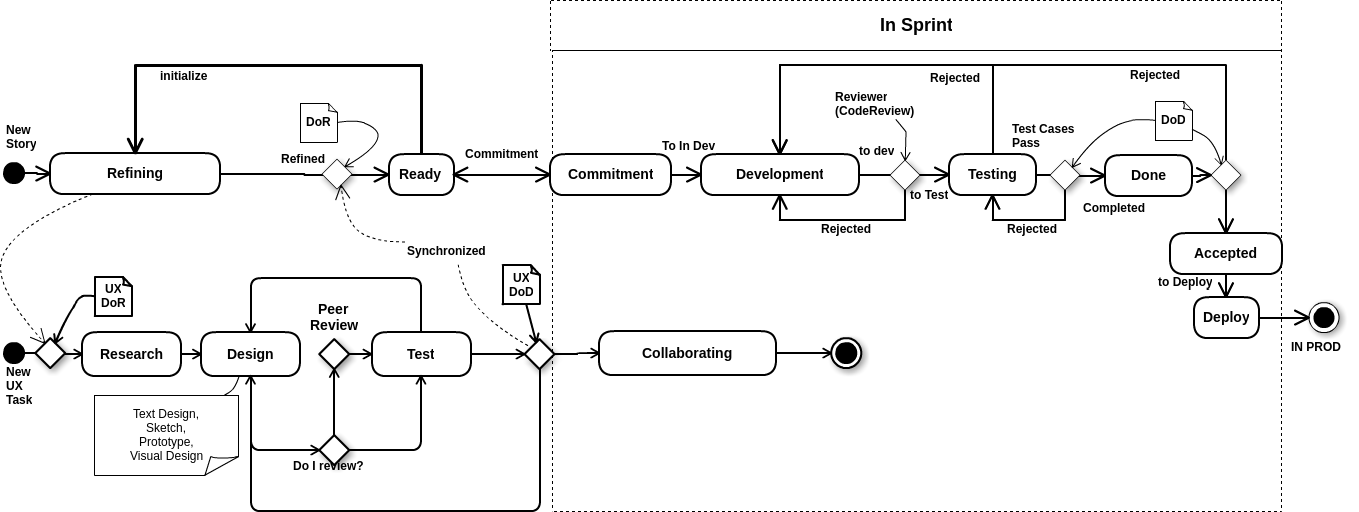
\includegraphics[width=1\textwidth]{UXtask-and-Story-in-Scrum}
  \caption{Ejemplo de coordinación entre flujos de tarea UX e historia}
  \centering
  \label{fig:UXtask-and-Story-in-Scrum} %\ref{fig:UXtask-and-Story-in-Scrum}
\end{figure}

\subsection{DevOps}

La integración a escala para que una Software Factory sea ágil y lleve adelante uno de sus principios, el Continuous Delivery, es lo que se denomina DevOps. DevOps es la integración de Ingeniería de Desarrollo de Software con la Ingeniería de Operaciones, que es todo el soporte IT y de plataforma para posibilitar que el proceso de desarrollo sea ágil, haciendo entregas frecuentes de calidad y logrando la colaboración entre el personal de desarrollo y el personal de operaciones a lo largo de todas las etapas del ciclo de vida de producción de software. DevOps es una parte central del agilismo en la entrega de software eficiente, por medio de la integración de equipos, metodologías ágiles, técnicas y stack tecnológico como una sola organización. El objetivo principal de DevOps es minimizar los cuellos de botella en el pipeline de entrega, haciéndolo más eficiente y ágil \footnote{\cite{DevOps-for-dummies-2015}}.

\begin{figure}[h]
  \centering
  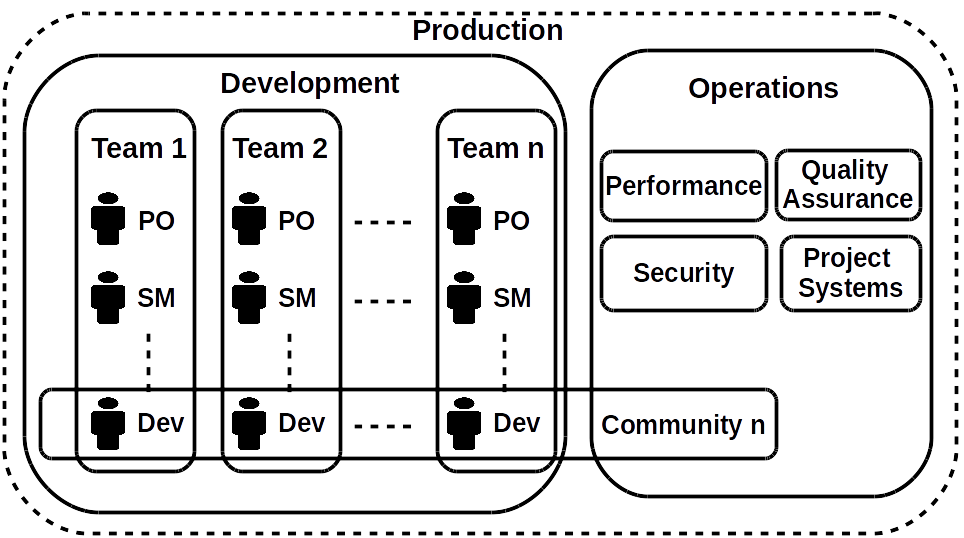
\includegraphics[width=0.80\textwidth]{DevOps}
  \caption{Ejemplo de integración de equpos en DevOps}
  \centering
  \label{fig:DevOps} %\ref{fig:DevOps}
\end{figure}

Una manera de integrar Operaciones con Desarrollo es mediante el uso de herramientas compartidas, misma cultura, comunidades en común, procesos ágiles compartidos, comunicación estandarizada, etcétera. Algo crucial en una organización madura es la automatización máxima en procesos de Continuous Integration y Continuous Delivery.

En cuanto a Scrum, el área de operaciones no necesita implementar Scrum, pero sí puede llevar en práctica sus valores, ser ágil (con Lean, Kanban, DAD, etc.) y tener en cuenta los ciclos Scrum de los equipos de desarrollo. DevOps es sólo un paso importante para unirse a la cultura general de la colaboración ágil y que debe involucrar a todas las disciplinas en una organización. 


\section{Modelos de escalamiento}

Existen diversos modelos, marcos y frameworks para escalamiento como lo son el modelo Spotify, SAFe, LeSS, Nexus, DAD, Lean Management, Agile Portfolio Management (APM), Recipes for Agile Governance in the Enterprise (RAGE) y otros. A continuación una breve reseña de algunos de ellos.

\subsection{Spotify}

Spotify es un caso de estudio que demuestra que puede ser aplicado más allá de pequeñas empresas o startup, sino en empresas más grandes (Spotify constaba en 2014 de aproximadamente de 250 personas en tres países). Por este motivo es un modelo de referencia. El modelo de Spotify consta de equipos escuadrones (squad), equivalentes a Equipos Scrum, con un PO y un SM llamado también Team Facilitator (Coach del equipo). Los escuadrones relacionados se agrupan en tribus (tribe) de no más de 100 personas, conformando un área de producto (como por ejemplo un tipo de producto) o área funcional (como por ejemplo infraestructura). La tribu tiene un líder de tribu (Tribe lead) quien se encarga de asegurar un alto rendimiento de la tribu, dar soporte a los líderes de los capítulos, facilitar y entrenar a los SM y construir liderazgo dentro de la tribu. 

\begin{figure}[h]
  \centering
  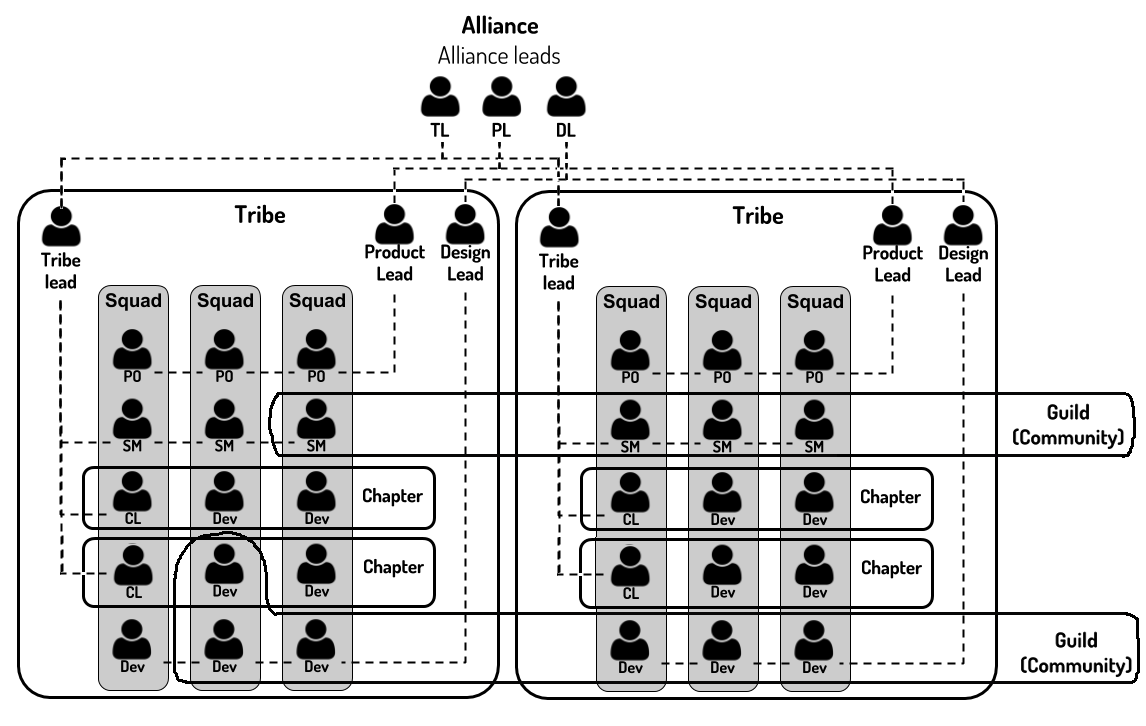
\includegraphics[width=0.99\textwidth]{Spotify_organizational_model}
  \caption{Modelo organizacional Spotify}
  \centering
  \label{fig:Spotify_organizational_model} %\ref{fig:Spotify_organizational_model}
\end{figure}

La tribu también tiene un líder de producto (PL) y uno de diseño (DL). Dentro de cada tribu hay capítulos (Chapter) y cada uno engloba un área funcional técnica de ingeniería, agrupando a los miembros de diferentes escuadrones con habilidades similares y que trabajan dentro del mismo área de competencia (por ejemplo el capítulo QA, BE, FE, etc.). Cada capítulo tiene un líder del capítulo ("Chapter lead" o CL) quien se encarga del desarrollo profesional, la cultura de la ingeniería, el apoyo del escuadrón y en asegurar la contratación de las personas adecuadas. Los líderes de capítulo suelen ser desarrolladores a tiempo parcial, por lo general se sientan en uno de los escuadrones de la tribu. 
Las diferentes tribus se pueden relacionar de diferentes maneras. Dos de ellas son la alianza (Alliance) y las comunidades (Guild). Una comunidad es una "comunidad de interés" (explicadas anteriormente). Los capítulos siempre son locales para una tribu, mientras que una comunidad generalmente es transversal a varias tribus. Cada comunidad puede tener un "coordinador de comunidad" y su alcance es más flexible. Y por último, la alianza une a diferentes comunidades por cohesión funcional de producto y tiene tres líderes serviciales (TL, PL y DL) quienes facilitan el trabajo de los líderes de las tribus unidas y el funcionamiento de las tribus, en general.

\subsection{SAFe}

El framework Scaled Agile Framework o SAFe consiste en una base de conocimientos de patrones integrados modulares, por niveles organizativos, destinados al desarrollo Lean-Agile a escala empresarial. Scrum se integra en SAFe en el primer nivel inferior organizativo, el nivel de equipo. A este nivel le siguen los niveles de programa, flujo de valor y portafolio. SAFe propone elementos opcionales de integración, un nuevo rol llamado Product Manager quien dirige a los POs de los equipos, otro nuevo rol llamado Release Train Engineer quien coordina a los SMs, la coordinación de backlogs por medio de un Backlog a nivel programa y la coordinación entre equipos por medio de eventos conjuntos y refinamientos, eventos trimestrales, System Team, Scrum of Scrums, Team Backlog y Team PO. SAFe propone que los equipos deben tener sus iteraciones sincronizadas y a tiempos periódicos deben tener una iteración de integración y planificación de todos los equipos o productos  (se planifican trenes de releases). Para más información hay que remitirse a la guía y definición de prácticas dada por el sitio web de SAFe.

\subsection{LeSS}

Por otro lado tenemos al framework Large-Scale Scrum o LeSS que  es un marco de desarrollo de productos que extiende Scrum con reglas de escalado y directrices sin perder los propósitos originales de Scrum. LeSS tiene un conjunto de principios alineados a Scrum y sumado el pensamiento sistémico. Además tiene alrededor de 28 reglas disponibles en 3 libros y propone diferentes mecanismos de coordinación como eventos conjuntos y refinamiento, CoP, SoS, Integración de código, feature teams y Area Product Owner. LeSS también propone subdivisiones de la organización por áreas de valor o Customer Value. Para más información hay que buscar en la guía del sitio web “less.works” y en diferentes libros que tratan el tema, como por ejemplo: Large-Scale Scrum, More with LeSS de Craig Larman y Bas Vodde.

\subsection{Modelo Nexus}

Nexus es un marco de trabajo para desarrollar y mantener iniciativas a escala de desarrollo de productos y software basado en Scrum. Fue creado por Ken Schwaber y Scrum.org. Es un exoesqueleto cuyo corazón es un conjunto de Equipos Scrum combinados para crear un Incremento Integrado, usando una única Lista de Producto Backlog, manteniendo "Listas de Pendientes" por Sprint y apoyados por un "Equipo de Integración Nexus" quien brinda soporte para asegurar que se produzca un Incremento Integrado. Para más información basta leer la "Guía Nexus" publicada en Scrum.org.

\subsection{DAD}

El marco de decisiones de procesos “Disciplined Agile Delivery” o DAD, brinda una orientación ligera para ayudar a las organizaciones a escalar agilidad y buscar optimizar sus procesos de tecnología de la información (IT) de una manera sensible al contexto ágil y DevOps. Para ello, muestra cómo las diversas actividades, como la entrega de soluciones, las operaciones, la arquitectura empresarial, la gestión de cartera y otros equipos y áreas trabajan juntas. Las reglas implicadas en este marco hacen que la empresa busque ser consciente y escalable. La referencia primaria para DAD es el libro “Disciplined Agile Delivery: A Practitioner's Guide to Agile Software Delivery in the Enterprise”,  escrito por Scott Ambler y Mark Lines.\newline
\newline

Si bien estos modelos tiene distintos grados de aceptación y éxito en muchas organizaciones, no se deben tomar como ley en piedra aplicándolos en cualquier contexto u organización. No se deberían implementar como recetas a seguir o soluciones ideales a implantar. Para aplicarlos en una organización deben ser evaluados y, en caso de aplicar alguna de sus pautas, ajustados según contexto y necesidades. Se recomienda aplicar también el pensamiento sistémico, ingeniería de sistemas y perspectivas de otras disciplinas.

\section{Equipo de mejora continua}

Como se ha visto, el escalamiento no es tarea simple y no existe una solución universal. Se puede dejar que los cambios organizacionales emerjan de abajo hacia arriba (desde los equipos, comunidades o individuos), sean dirigidos por un ente director (coaches, consultoras o un líder transformacional) o algo mixto. Hay frameworks que recomiendan que, cuando se desea llevar a cabo transformaciones organizacionales hacia la agilidad, se constituya un equipo de expertos ágiles llamado centro de excelencia, centro de transformación digital, centro de soporte ágil o equipo transversal de mejora continua \footnote{ScrumStudy recomienda un Scrum Guidance Body y DAD recominda un equipo de excelencia CoE.}. Este equipo se encargaría de hacer coaching a equipos y a otros roles, proponer iniciativas de mejoras organizacionales y apoyar la transformación cultural. El equipo puede estar formado por Coaches Ágiles Empresariales, gerentes ágiles, ingenieros de sistemas, ingenieros de operaciones, capital humano, etc. Los miembros deben ser capaces de trabajar en cualquier nivel de la organización, teniendo una visión multidisciplinaria, global y perspectiva sistémica.
          % Scaling to big organizations
\chapter{Complementos de Scrum}

Scrum no tiene como objetivo dar instrucciones precisas a los equipos sobre la forma concreta en la que deben llevar a cabo su desarrollo. Scrum espera que los equipos hagan lo que sea necesario para ellos para entregar el producto de calidad. Las prácticas y herramientas de desarrollo cambian y mejoran de manera continua y los buenos equipos trabajarán constantemente en pos de obtener el mejor uso de las mismas. Desde esta perspectiva, se puede consensuar en un anillo de complementos útiles que rodea el núcleo de Scrum y que pueden potenciar el trabajo ágil y la práctica de ingeniería. Estos complementos son métodos y técnicas complementarias a Scrum, sujerencias y recomendaciones, lecciones aprendidas y conceptos aledaños. En este capítulos trataremos estos temas.

% Malas prácticas, consejos, tecnicas complementarias, casos de estudios

%Técnicas para requerimientos
% Historias de usuarios
% Técnica Killen :  sirve para definir cuales son las cuestiones clave a desarrollar en un proyecto y su priorización logrando un conjunto de historis de usuario.
% Mapas de historia (Técnica propuesta por Jeff Patton)
% Articles: The New User Story Backlog is a Map By Jeff Patton. JPattonAssociates.com, Octuber 8, 2008.
% URL: http://jpattonassociates.com/the-new-backlog/
%Técnicas de Planeación
%Técnicas de estimación
% Poker de planeación
%Técnicas de Comunicación
% Radiadores de información
% Scrum task board
% Comunicación osmótica
% -----------técnica que te permita limitar la cantidad de trabajo en progreso y la priorización de las tareas, como % son la Técnica pomodoro y la Matriz de Eisenhower respectivamente.
%Técnicas de Programación

\newpage
\section{Técnicas para requerimientos}

\subsection{Historias de usuarios}

Para Scrum las hipótesis de requerimientos se representan en items de Backlog de producto PBI. A estos PBIs se los suele denominar "Story" o "Historias de Usuarios"\footnote{Las "User Story" son una técnica de eXtremme Programming (XP)}. El Product Backlog incluye incisos o Stories que aportan valor al cliente y que suelen ser descripción de requisitos funcionales. Aunque también puede incluir entradas para exploración de características, necesidades del cliente u opciones técnicas, requerimientos no funcionales, el trabajo necesario para lanzar el producto, y otros incisos, así como la configuración del entorno o arreglar defectos \footnote{\cite{Scrum-Institute-2015}}. O sea que puede proporcionar valor en forma indirecta mediante el aumento de la calidad o la reducción de los incidentes en el largo plazo \footnote{\cite{Scrum-Institute-2015}}.

Las historias representan un concepto verificable y simple, que el Product Owner quiere implementar en el producto. Según el concepto general de metodología Ágil, la historia se define como una "promesa de una conversación" o una "descripción de una característica" \footnote{\cite{UNTREF-2014}, \cite{Dan-North-2015}}. Según esta perspectiva, la historias de usuario representa una "funcionalidad de aplicación" para un usuario y que brinda un beneficio (ROL + FUNCIONALIDAD + BENEFICIO). Las mismas se escriben siempre con lenguaje de negocio y respetando la siguiente pauta de estructura:\newline

\textbf{COMO} <ROL> \textbf{QUIERO} <FUNCIONALIDAD> \textbf{PARA QUE} <BENEFICIO>\newline

Por ejemplo:

%Example of User Story
\begin{itemize}
\item \textbf{COMO} ScrumMaster 
\item \textbf{QUIERO} que las reuniones no se extiendan más de un tiempo consensuado 
\item \textbf{PARA QUE} no se pierda el foco.
\end{itemize}

La historia de usuario no es exactamemte un requerimiento, pero puede considerarse como el título de una hipótesis de requerimiento como recordatorio de algo relevante a conversar con el usuario o cliente. En consecuencia lo relevante es su evolución como conversación \footnote{\cite{UNTREF-2014}}.

La historia de usuario describe lo que el usuario quiere hacer desde la perspectiva de una interacción con un proceso de negocio, describe el objetivo del usuario en términos de necesidad de obtener algo que se hace en el negocio \footnote{\cite{Scott-Bellware-2008}}.

Según Dan North y en el marco de Behavior-Driven Development (BDD), una Story es más un requerimiento, pues tiene que ser una descripción de un requisito y su beneficio para el negocio, y un conjunto de criterios con los que todos estamos de acuerdo de qué es o lo que se hace, "lo que el cliente necesita" \footnote{\cite{Dan-North-2015}}. 

\subsubsection{Criterio de demarcación}

Las historias de usuario bien escritas son esenciales para el desarrollo ágil y la ingeniería de software. Existen ciertas características a tener en cuenta a la hora de escribir una historia de usuario y determinar cuál es una bien escrita o una válida. El criterio de demarcación aceptado en metodología ágil en general es el criterio INVEST\footnote{INVEST es un acrónimo creado por Bill Wake.} y que consta de seis características a cumplir \footnote{\cite{UNTREF-2014}, \cite{Scrum-Alliance-2015}}:

\begin{enumerate}

\item \textbf{Independiente:} una historia debe ser atómica. Es decir que se debe buscar asegurar la cohesión funcional y el bajo acoplamiento entre historias distintas. La fuerte dependencia entre diferentes historias hace que sea más dificil planificar, priorizar y estimar.

\item \textbf{Negociable:} debe ser conversable y en consecuencia negociable (es viva). Las historias "no son requerimientos contractuales"\footnote{"Las user stories no son obligaciones contractuales"\cite{Cohn-2004}} ni requisitos rígidos, y su detalle y precisión debe poder evolucionar en el tiempo en procesos de refinamiento y conversaciones en una ingeniería de requerimientos evolutiva.

\item \textbf{Valueble:} debe generar un valor al cliente (usuario o comprador). Una Story sin una declaración de la motivación del usuario a menudo se piensa que es no accionable; es decir, la historia no se puede estimar o implementar fácilmente \footnote{\cite{Scott-Bellware-2008}}. Lo ideal, además de la declaración explícita del beneficio, es que haya una forma de medir el valor que aporta al cliente.

\item \textbf{Estimable:} se debe poder estimar. La historia debe brindar la suficiente información que de la certidumbre necesaria para que los desarrolladores puedan estimarla y permitir, de este modo, que se pueda priorizar y planificar. 

\item \textbf{Pequeña:} debe ser lo suficientemente pequeña para entrar en un sprint o iteración. El tamaño pequeño de las historias ayuda a reducir el tamaño del lote, incrementar el flujo de valor hacia el cliente y asegurar que cada miembro del equipo de desarrollo pueda hacer una contribución valiosa cada día. Por ejemplo, en cada Sprint se podrían completar entre cuatro y ocho historias pequeñas. A medida que una historia es más grande va a tener más errores asociados a la estimación y alcance, y aumentará la probabilidad de terminar en un Sprint fallido.

\item \textbf{Probable:} debe poder permitir la contrastabilidad. La contrastabilidad del enunciado de la historia es la propiedad de ésta de ser capaz de ser sometida a una prueba empírica y repetible a fin de evaluar su adecuación o no a los hechos a los que se refiere o resultados esperados. Esta característica es crucial para hacer ingeniería, sin la contrastabilidad no se hace ingeniería. Un ejemplo de historia no probable sería: "Como usuario quiero un software hermoso y facil de usar".

\end{enumerate}

\subsubsection{¿Qué NO es una Historia de Usuario?}

Si no cumple con el criterio INVEST es bastante probable que no sea una Story. Por ejemplo una tarea puramente técnica (que le interesa solo al desarrollador), un refactoring técnico o un Spike no cumplen con INVEST y en su generalidad no son Story. 
Veamos los siguientes ejemplos:

\begin{itemize}

\item \textbf{Spike:}
No es una Story ya que es una tarea de investigación y/o experimentación en formato time-boxing por lo que no cumple con ser probable ni estimable (no cumple con dos criterios).

\item \textbf{Refactoring Task:}
Es una tarea técnica de reingeniería que no es valuable o su valoración es a futuro o en relación a un atributo de calidad que puede no estar directamente solicitado por el cliente o no impacta en beneficio inmediato para el cliente, ya que podría estar resolviendo una "deuda técnica"\footnote{Deuda técnica es la incurrida involuntariamente debido a trabajos de baja calidad o deuda incurrida intencionalmente (McConnell, Ward Cunningham) y que consta en arquitectura no escalable, defectos en el código, documentación inservible o desactualizada, problemas para migrar o actualizar funcionalidades o problemas por falta de mantenimiento.}. Esto no quiere decir que no pueda haber una "story de refactoring" que puede proporcionar valor en forma indirecta mediante el "aumento de la calidad o la reducción de los incidentes en el largo plazo".

\item \textbf{Technical Story:}
“Cada historia tiene que ser valorada por los usuarios. Pero eso sería un error."\footnote{\cite{Cohn-2004}} Pues en realidad, una historia de usuario describe la funcionalidad que será valiosa para un usuario o comprador de un sistema o software \footnote{\cite{Cohn-2004}}. Hay historias que especifican aspectos técnicos que no son valiosos para el usuario sino mas bien para el cliente o comprador (la valoración es transitiva y no directa). Historias técnicas pueden ser valorados por los compradores que contemplan la compra del producto, pero no serían valorados por los usuarios reales. Pero esto no es lo que podemos llamar una "Technical Story" sino que es una Story con aspectos técnicos que tiene valor para el cliente. Para Scott Ambler en Agile Modeling, una Story es una definición de muy alto nivel de un requerimiento que puede ser funcional o no, por ejemplo de un requerimiento técnico \footnote{\cite{Scott-Ambler-2015}}, por ejemplo: "como usuario quiero que las transcripciones estén disponibles en línea a través de un navegador estándar lo que me permite acceder desde cualquier lugar"\footnote{\cite{Scott-Ambler-2015}}.

Cuando se habla de "Technical Story" se referencia a aquella historia técnica que sólo es valorada por los desarrolladores. Estas historias son las que se quieren evitar y considerar como Technical Story que podría ser una tarea técnica o una historia mejor redactada. Este tipo de historias se centran en la tecnología y las ventajas para los programadores. Es muy posible que las ideas detrás de estas historias sean buenas, pero en cambio deben ser escritas para que los beneficios a los clientes o usuarios sean evidentes. Esto permitirá que el cliente priorizar inteligentemente estas historias en el calendario de desarrollo \footnote{\cite{Cohn-2004}}.

Para la Agile Alliance una Story no se corresponde en general a un "componente técnico" o de la "interfaz de usuario", pues a pesar de que a veces puede ser un atajo útil hablar de por ejemplo "la historia de diálogo de búsqueda", pantallas, cuadros de diálogo y botones, no son historias de usuario \footnote{\cite{Scrum-Alliance-2015}}.

\end{itemize}

\subsubsection{Componentes de una Historia de Usuario}

Las historias de usuarios se componen de tres elementos comunmente denominados las tres 'C'\footnote{Las 3 Cs de Ron Jeffries.}:

\begin{enumerate}

\item \textbf{Carta o tarjeta (Card):} Las historias se deben poder escribir en una tarjeta de papel pequeña. Por ese motivo la redacción de las mismas debe ser clara, precisa y concisa para caber en una tarjeta de papel.

\item \textbf{Conversación:} Las historias deben tener y generar conversaciones cara a cara entre el Product Owner y el Equipo de Desarrollo.

\item \textbf{Confirmación:} Deben estar suficientemente explicada para que el Equipo de Desarrollo qué es lo que se desea construir y qué es lo que se espera como resultado de dicha implementación. La confirmación es el "Criterio de Aceptación" que los desarrolladores deben tener en cuenta para que la misma sea aceptada por el cliente.

\end{enumerate}

\subsubsection{Criterio de Aceptación}

Las historias de usuario tienen límites específicos para las características del producto, proceso o servicio definido en la hipótesis de requerimiento que determinan los resultados esperados para que la historia sea aceptada por el cliente. En otras palabras, el criterio de aceptación es el conjunto de afirmaciones útiles para que el cliente valide la historia.

La estructura de un criterio de aceptación presentado como escenario puede ser como la siguiente:

%Criterio de aceptación ejemplo con un escenario
\begin{itemize}
\item \textbf{Scenario 1:} Título
  \begin{itemize}
  \item \textbf{Given} [contexto] And [otro contexto]...
  \item \textbf{When}  [evento] 
  \item \textbf{Then}  [resultado] And [otro resultado]...
  \end{itemize}
\end{itemize}
  
\newpage
\section{Técnicas de Estimación}

\subsection{Puntos de historia}

Los puntos de historia o "Story Points" son una medida relativa de estimación de una historia de usuario para poder medir su tamaño y útil para medir la velocidad de un equipo. Se usa para hacer estimaciones relativas, que quiere decir que las historias se comparan entre si, buscando mantener una relación proporcional entre ellas según sus puntos de historia. O sea que si se piensa a nivel de esfuerzo, una historia que tiene 3 puntos de historia requerirá tres veces más de esfuerzo que una que sea de un punto historia.

Hay que tener en cuenta que "bajo ningún punto de vista la estimación (en story points) es un compromiso"\footnote{\cite{UNTREF-2014}} y que los puntos de historia no son medidas objetivas convertibles en forma precisa a horas. Justamente se usan puntos de historia para no estimar en horas hombre.

\subsection{Poker de planeación}

El Poker de planeación o "Planning Poker"\footnote{El "Planning Poker" proviene de un paper presentado por James Greening llamado "cómo evitar análisis parálisis en la planificación de liberaciones"\cite{James-Grenning-2002} donde se basa en el método Wideband Delphi para realizar la estimación de requerimientos de forma colaborativa. Luego el método fue popularizado por Mike Cohn con su libro "Agile Estimating and Planning"\cite{Cohn-2005}} es una técnica de estimación y planificación ágil que se basa el consenso por sabiduría de grupo. 

La dinámica consiste en que el Product Owner inicia leyendo una historia de usuario ágil o describe una característica para los desarrolladores estimadores. Cada estimador posee una baraja de "Cartas de Poker de Planificación". Los valores representan el número de puntos de la historia, día ideal, u otras unidades en las que el equipo estima. Los estimadores discutir la función, haciendo preguntas al Product Owner, según sea necesario. Cuando la función se ha discutido plenamente, cada estimador selecciona de forma privada una tarjeta a representar a su estimación. Todas las tarjetas se revelaron a continuación, al mismo tiempo. Si todos los estimadores seleccionan el mismo valor, que se convierte en la estimación. Si no, los estimadores discuten sus estimaciones. Los estimadores de valores altos y bajos deben compartir sus razones. Tras un nuevo debate, cada estimador vuelve a seleccionar una tarjeta de estimación, y todas las tarjetas se revelan de nuevo al mismo tiempo. El proceso se repite hasta que se logre el consenso, o hasta que los estimadores deciden que la estimación ágil y planificación de un ítem en particular debe ser diferida hasta que la información adicional se puede adquirir.


\subsubsection{Cartas de Poker de Planificación}

Las Cartas de Poker de Planificación que más se usan son las de Fibonacci y las de talles de remeras:

\begin{enumerate}

\item \textbf{Talles de remeras:} Las cartas de talles contempla los valores XS (muy pequeño), S (Pequeño), M (Mediano), L (grande), XL (muy grande) y XXL (extra grande). Estos valores sirven para estimar épicas, tamaños de historias o trabajo a alto nivel. 

\item \textbf{Fibonacci:} Las cartas Fibonacci contempla los valores 0, 1, 2, 3, 5, 8, 13, 20, 40 y 100, que es la secuencia fibonacci que se suele recomendar. Estos valores son útiles para estimar complejidad de historias o trabajo a nivel medio. Realizando una estimación relativa, estos valores corresponden a puntos de historia.

\end{enumerate}

\newpage
\section{Técnicas de Comunicación}

\subsection{Hacer silencio}

Una técnica para lograr silencio en un grupo es pedir silencio cuando se levanta la mano, los que ven la mano levantada tienen que callarse y levantar a su vez la mano. Cuando cualquiera ve a alguien con la mano levantada se debe callar y a su vez levantar la mano. Este comportamiento se termina propagando rápidamente en todos los integrantes hasta que se logra el silencio. Es una técnica muy útil en la reuniones cuando las personas se dispersan comunicándose en forma caótica o cuando alguna actividad de conversación libre se extiende del tiempo necesario.


\subsection{Gestión visual}

La gestión visual es la utilización de elementos y técnicas visuales, como complemento de Scrum, para la organización del trabajo y la irradiación visual del trabajo. Es aconsejable que los irradiadores de información presenten las siguientes características:

\begin{enumerate}

\item \textbf{Ubicación ostensible:} estar ubicado en el lugar de trabajo en forma de afiches, carteles o pizarras visibles.

\item \textbf{Soporte físico:} estar hechos de material tangible como papel en vez de usar software, salvo el caso de monitores grandes.

\item \textbf{Resumen autoexplicativo:} contener información importante autoexplicativa y didáctica.

\end{enumerate}

Ejemplos de irradiadores de información son: el gráfico burndown, indicadores de estados del build (usando semáforos), métricas de errores, riesgos activos, impedimentos. etcétera.

\subsection{Tableros Scrum/Kanban}

El tablero Scrum/Kanban o "Scrum Kanban Board" es una técnica que consiste en utilizar un tablero Kanban (ver figura \ref{fig:ScrumKanbanBoard}), como irradiador de información, para el manejo del cilo de estados de las tareas y de los impedimentos. El tablero Kanban debe ser visible por todo el equipo y por lo tanto transparente para todos los involucrados. Por ejemplo, durante una Daily Scrum todo el equipo es capaz de ver qué tareas se resuelven, cuáles no se han abordado todavía y qué impedimentos existen.

\subsubsection{Ejemplo de un Scrum kanban board}

Ver figura \ref{fig:ScrumKanbanBoard}.

\begin{figure}[h]
  \centering
  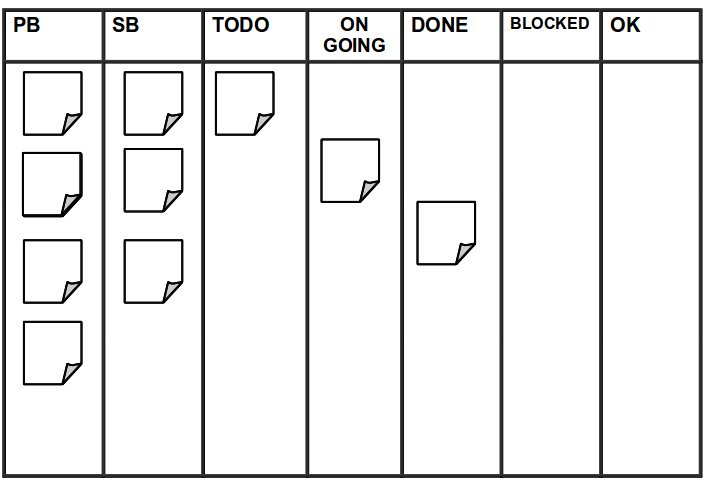
\includegraphics[width=0.9\textwidth]{ScrumKanbanBoard}
  \caption{Tablero Kanban para Scrum}
  \centering
  \label{fig:ScrumKanbanBoard} %\ref{fig:ScrumKanbanBoard}
\end{figure}

\subsubsection{Ejemplo de un Scrum board}

Un Scrum board, Kamban Board o taskboard físico (Ver figura \ref{fig:ScrumBoard}) es una tabla donde se colocan postick representando tareas.

\begin{figure}[h]
  \centering
  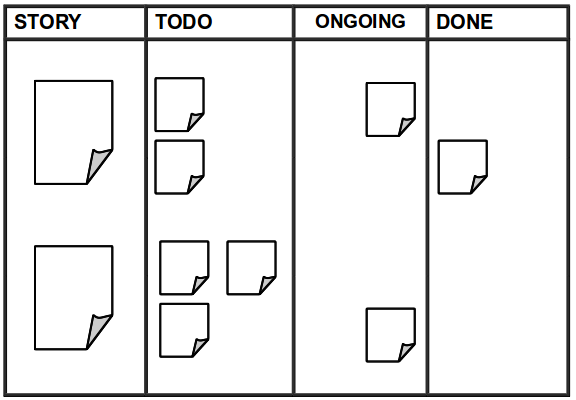
\includegraphics[width=0.8\textwidth]{ScrumBoard}
  \caption{Tablero Scrum}
  \centering
  \label{fig:ScrumBoard} %\ref{fig:ScrumBoard}
\end{figure}

\subsection{Tablero de Obstáculos}

El Tablero de Obstáculos (ver figura \ref{fig:ObstacleBoard}) es una herramienta visual útil para hacer seguimiento de los obstáculos o bloqueos del equipo que surgen en el trabajo del Sprint. El dueño del Tablero de Obstáculos es el Scrum Master, quien se encarga de buscar remover todos los obstáculos que puedan paralizar o ralentizar el trabajo del equipo o desviarlo de su foco esencial. El tablero tanbién le es útil al equipo para tener la visibilidad del estado de los obstáculos.

Ver figura \ref{fig:ObstacleBoard}.

\begin{figure}[h]
  \centering
  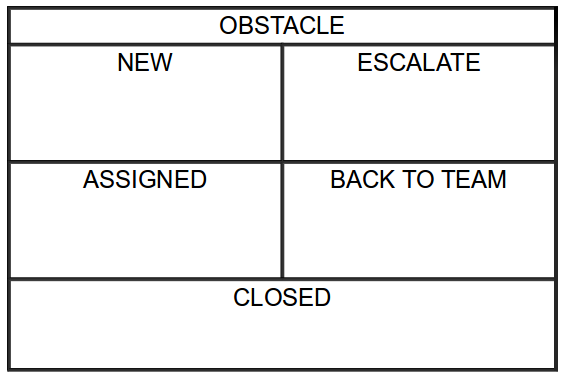
\includegraphics[width=0.6\textwidth]{ObstacleBoard}
  \caption{Tablero de Obstáculos}
  \centering
  \label{fig:ObstacleBoard} %\ref{fig:ObstacleBoard}
\end{figure}

\subsection{Gráficos de esfuerzo pendiente}

\subsubsection{Gráfico Burndown}

Un gráfico de trabajo pendiente o "Burndown charts"\footnote{El Burndown muestra la cantidad de trabajo que queda. \cite{SBOK-2013}} (figura \ref{fig:Burndown_chart}) es uno que muestra el trabajo restante ("Remaining Scope") o que queda por hacer versus tiempo. Muestra la velocidad a la que se están completando los PBIs o historias reflejando el avance y permitiendo extrapolar si el Equipo podrá completar el trabajo en el tiempo restante.

\begin{figure}[h]
  \centering
  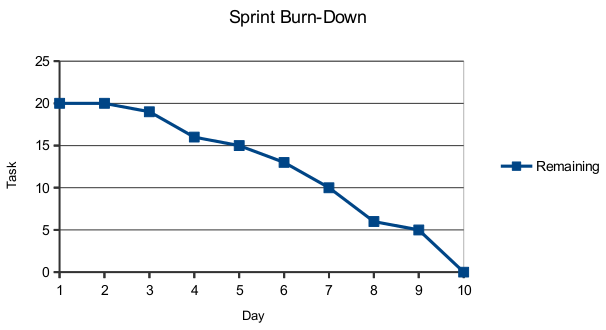
\includegraphics[width=0.9\textwidth]{Burndown_chart}
  \caption{Gráfico Burndown}
  \centering
  \label{fig:Burndown_chart} %\ref{fig:Burndown_chart}
\end{figure}

Se pueden utilizan dos gráficos de esfuerzo pendiente:

\begin{enumerate}

\item \textbf{Burndown de Sprint:} Días u horas pendientes para completar las tareas de la iteración (sprint burndown chart), realizado a partir de la lista de tareas de la iteración. Normalmente se utiliza para saber cuánto falta para terminar las historias comprometidas en un Sprint. Es un diagrama de dos ejes: en el eje X el tiempo en días de duración del sprint, en el eje Y la cantidad de trabajo comprometida con el cliente durante el sprint en las unidades que se hayan acordado.

\item \textbf{Burndown de Proyecto:} Días pendientes para completar los requisitos del producto o proyecto (product burndown chart), realizado a partir de la lista de requisitos priorizada (Product Backlog).

\end{enumerate}

\subsubsection{Gráfico Burn-Up}

El gráfico de trabajo realizado o Burn-up\footnote{El Burnup muestra el trabajo realizado como parte de la Sprint. \cite{SBOK-2013}} (figura \ref{fig:Burnup_chart}) es muy similar al Burndown, con la diferencia de que se parte del cero, y se va marcando la cantidad de trabajo completado en el Sprint. En este gráfico la curva va hacia arriba asercándose a una línea que representa el alcance comprometido. En este tipo de gráfico es más fácil visualizar los cambios de alcance.

\begin{figure}[h]
  \centering
  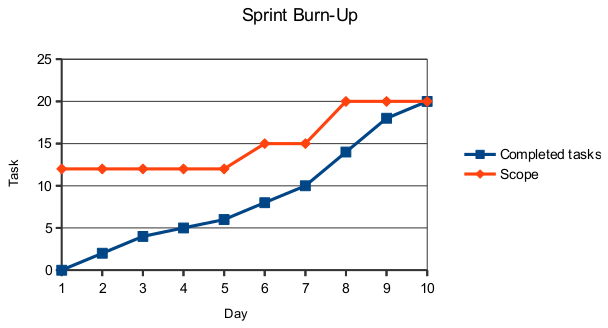
\includegraphics[width=0.9\textwidth]{Burnup_chart}
  \caption{Gráfico Burnup}
  \centering
  \label{fig:Burnup_chart} %\ref{fig:Burnup_chart}
\end{figure}

\newpage
\section{Técnicas de Programación}

Hay diferentes técnicas que pueden ser utilizadas en el proceso de desarrollo de software bajo el marco de Scrum. A continuación se describen algunas principales que sirven de soporte a metodologías ágiles:

\subsection{Técnica Pomodoro}

Se usa 'Pomodoro'\footnote{La Técnica Pomodoro es un método para la administración del tiempo desarrollado por Francesco Cirillo a fines de los años 1980\cite{Cirillo-Francesco-1980}.} como una técnica de gestión del tiempo y se basa en la hipótesis de que las pausas frecuentes en el trabajo pueden mejorar la agilidad mental. Por este motivo, la técnica consiste en dividir el tiempo dedicado a un trabajo en intervalos (time-boxing) de 25 minutos (llamados 'pomodoros') separados por descansos. Los primero tres descansos son de 5 minutos y el descanso despues del cuarto pomodoro es de 15 minutos, para luego repetir la secuencia en forma cíclica. Durante el intervalo pomodoro el trabajo debe ser focalizado, por lo que no se deben admitir distracciones o trabajos ajenos al trabajo principal. 
Esta es una técnica útil en el desarrollo ágil y en la programación en pareja (pair programming) además de otros contextos de trabajo.

\subsection{Programación de a pares}

La programación de a pares, “pairing” o “pair programming” consiste en que dos programadores participen conjuntamente en un esfuerzo combinado de desarrollo en un puesto de trabajo. La misma se puede extender al desarrollo de a pares (análisis, diseño, codificación, pruebas, diseño de interfaces de usuario, diseño gráfico, etc.).

Existen muchas razones por los que esta técnica es recomendable y las principales pueden ser las siguientes:

\begin{enumerate}

\item \textbf{Calidad:} Mejorar la calidad logrando reducir defectos por "revisión de a pares" mientras se programa.

\item \textbf{Aprendizaje:} Lograr el aprendizaje en equipo distribuyendo y nivelando el conocimiento. Pues, focalizarse en el aprendizaje es crucial para organizaciones scrum de equipos por características, donde todos deben manejar un conocimiento amplio y multidisciplinario. 

\item \textbf{Propiedad colectiva:}
Mejorar los diseños y las estimaciones debido a que todos tienen un conocimiento de la estructura del producto, un empoderamiento del mismo (propiedad colectiva del código) y de cómo puede impactar un cambio en parte de él.

\item \textbf{Resolución de problemas:} Permitir superar problemas difíciles de forma más simple, más rápido o al menos efectiva cuando trabajan juntos. La idea es que dos personas piensen mejor que una en resolver un problema.

\end{enumerate}

\subsection{Revisión de a pares}

La revisión de a pares o "peer review" es una práctica intrínseca de la actividad científica en un sistema de evaluación del trabajo científico, donde los miembros de la comunidad revisan los trabajos de sus pares\footnote{Formalmente el proceso de revisión por pares del trabajo científico fue iniciado en 1753 por la “Royal Society of London”.}. Por este motivo, implementar este tipo de prácticas en el desarrollo de software hace que sea una actividad ingenieril. El beneficio es lograr una mejor calidad y una reducción de defectos. Según Boehm "el 60 por ciento de los defectos de código se pueden eliminar durante las revisiones de a pares"\footnote{\cite{Boehm-2001}}. Así como en ciancia se revisan los trabajos de investigación antes de ser publicados, en ingeniería de software se revisa el código antes de ser desplegado.\newline
La práctica consiste en que una vez que el programador desarrolló un trabajo de codificación, solicite ante un colega compañero o un conjunto de ellos la inspección del código. Si se encuentran errores u observaciones, el desarrollador deberá mejorarlo y hasta que no tenga el visto afirmativo el código, no será desplegado o integrado al producto. Hay que tener en cuenta que para que la revisión por pares sea realmente productiva, debe ser ejecutada con el máximo de rigor, aunque implique retrasar despliegues de producto y no cumplir con los plazos comprometidos por el equipo. Cuando se aplica Scrum, el máximo de rigos incluye, además de la calidad del trabajo, prestar particular importancia al cumplimiento de la definición de terminado (DoD).

\subsection{Test Driven Development}

El "Test Driven Development" (TDD) o "desarrollo guiado por pruebas"\footnote{\cite{Jurado-2010}} es una práctica, técnica de desarrollo ágil y técnica de programación que hace foco en el comportamiento especificado de unidades de software\footnote{[Wikipedia 2014]} como disparador para el desarrollo de pruebas. Osea, basándose en especificaciones, esta práctica tiene como táctica escribir primero las pruebas (código de prueba) y después el código (código de producto) para luego realizar ciclos de "refactorización" \cite{Kent-Beck-2003}. Con este enfoque se pretende, entre otras cosas, que el diseño sea el código mismo (código de producto) y que las pruebas concretas (código de prueba) sirvan de documentación. Esta técnica se complementa con la automatización de pruebas. En todo ese conjunto de pruebas concretas, las pruebas de unidad se usan para validar métodos individuales y conjuntos de métodos. En consecuencia, en este tipo de desarrollos, se logran sistemas con un gran conjunto de pruebas (muchas líneas de código en pruebas).\newline
Si tenemos que asignar un lema a este enfoque es "la prueba en primer lugar" y su afirmación filosófica principal sería que "el diseño emerge del refactoring originado por pruebas".

\subsection{Integración contínua}

La integración continua (Continuous Integration\footnote{Continuous Integration fue propuesto inicialmente por Martin Fowler.}) es un modelo informático que consiste en hacer integraciones automáticas de un proyecto, compilación y ejecución de pruebas, lo más a menudo posible para así poder detectar fallos cuanto antes.
    % Complement or additionals
\chapter{Glosario y Acrónimos}

\begin{table}[h]
\begin{tabular}{lllll}
\cline{1-2}
\multicolumn{1}{|l|}{Nombre}   & \multicolumn{1}{l|}{Descripción}  &  &  &  \\ \cline{1-2}
\multicolumn{1}{|l|}{Artifact}   & \multicolumn{1}{l|}{Artefacto o almacén de incisos de trabajo}  &  &  &  \\ \cline{1-2}
\multicolumn{1}{|l|}{BDUF}   & \multicolumn{1}{l|}{Gran diseño al inicio (Big Design Up Front)}  &  &  &  \\ \cline{1-2}
\multicolumn{1}{|l|}{DoD}   & \multicolumn{1}{l|}{Definición de terminado (Definition of Done)}  &  &  &  \\ \cline{1-2}
\multicolumn{1}{|l|}{DoR}   & \multicolumn{1}{l|}{Definición de completitud (Definition of ready)}  &  &  &  \\ \cline{1-2}
\multicolumn{1}{|l|}{DT}   & \multicolumn{1}{l|}{Equipo de desarrollo (Development Team)}  &  &  &  \\ \cline{1-2}
\multicolumn{1}{|l|}{DUF}   & \multicolumn{1}{l|}{Diseño al inicio (Design Up Front)}  &  &  &  \\ \cline{1-2}
\multicolumn{1}{|l|}{Features}   & \multicolumn{1}{l|}{
\begin{tabular}[c]{@{}l@{}}
Representan interacciones y acciones del usuario con\\ 
el sistema. \\ 
Son funcionalidades que entregan valor de cara al usuario.\\
\end{tabular}
}  &  &  &  \\ \cline{1-2}
\multicolumn{1}{|l|}{MMP}   & \multicolumn{1}{l|}{(Minimal Marketable Product) Producto comerciable mínimo.}  &  &  &  \\ \cline{1-2}
\multicolumn{1}{|l|}{MVP}   & \multicolumn{1}{l|}{(Minimal Viable Product) Producto viable mínimo.}  &  &  &  \\ \cline{1-2}
\multicolumn{1}{|l|}{PB}   & \multicolumn{1}{l|}{Backlog de producto (Product Backlog)}  &  &  &  \\ \cline{1-2}
\multicolumn{1}{|l|}{PBI}   & \multicolumn{1}{l|}{Ítem de PB (Product Backlog Item)}  &  &  &  \\ \cline{1-2}
\multicolumn{1}{|l|}{PI}   & \multicolumn{1}{l|}{Incremento de producto (Product Increment)}  &  &  &  \\ \cline{1-2}
\multicolumn{1}{|l|}{PMI}   & \multicolumn{1}{l|}{
\begin{tabular}[c]{@{}l@{}}
Instituto de Gestión de Proyectos \\
(Project Management Institute) \\
\end{tabular}
}  &  &  &  \\ \cline{1-2}
\multicolumn{1}{|l|}{PO}   & \multicolumn{1}{l|}{Dueño del producto (Product Owner)}  &  &  &  \\ \cline{1-2}
\multicolumn{1}{|l|}{ROI}   & \multicolumn{1}{l|}{Retorno de la inversión (Return On Investment)}  &  &  &  \\ \cline{1-2}
\multicolumn{1}{|l|}{SCRUM}   & \multicolumn{1}{l|}{
\begin{tabular}[c]{@{}l@{}}
Es un juego de rugby en el que, por lo general, tres\\
miembros de cada línea se unen opuestos unos a \\
otros con un grupo de dos y un grupo de tres \\
jugadores detrás de ellos, lo que hace un grupo \\
de ocho personas, tres, dos, tres formados en cada \\
lado; el balón se deja entre la línea divisoria de \\
ambos grupos, los jugadores están abrazados \\
y tomados de la cintura de un compañero de equipo\\
y los del frente hombro a hombro con el oponente,\\
y se trata hacer fuerza grupalmente para desplazar \\
al grupo rival y patear la pelota hacia atrás para \\ 
que un compañero de equipo la tome.\\
\end{tabular}
}  &  &  &  \\ \cline{1-2}
\multicolumn{1}{|l|}{SB}   & \multicolumn{1}{l|}{Backlog de iteración (Sprint Backlog)}  &  &  &  \\ \cline{1-2}
\multicolumn{1}{|l|}{SM}   & \multicolumn{1}{l|}{Facilitador (ScrumMaster)}  &  &  &  \\ \cline{1-2}
\multicolumn{1}{|l|}{SOA}   & \multicolumn{1}{l|}{
\begin{tabular}[c]{@{}l@{}}
Arquitectura Orientada a Servicios \\
(Service-Oriented Architecture) \\
\end{tabular}
}  &  &  &  \\ \cline{1-2}
\multicolumn{1}{|l|}{SP}   & \multicolumn{1}{l|}{Iteración (Sprint)}  &  &  &  \\ \cline{1-2}

%% Ejemplo de como agregar una fila con saltos de linea
%% \multicolumn{1}{|l|}{Example}   & \multicolumn{1}{l|}{
%% \begin{tabular}[c]{@{}l@{}}
%% texto texto texto texto texto texto texto  \\
%% texto texto texto texto texto texto texto \\
%% \end{tabular}
%% }  &  &  &  \\ \cline{1-2}

                           &                                                          &  &  & 
\end{tabular}
\end{table}
 % Dictionary

% Bibliography
\bibliographystyle{apalike}
\bibliography{content/bibliography_list}

% License message
% Creative Commons by-sa 4.0  

\vspace{1cm} %1cm vertical space
\hspace{1cm}\newline %1cm horizontal space

\begin{center}
Los artículos y las ilustraciones de este libro se 
distribuyen bajo una licencia Creative Commons by-sa 4.0 
\newline


\includegraphics[width=0.3\textwidth]{license_CC_BY_SA_logo}
{\small 
\url{http://creativecommons.org/licenses/by-sa/4.0/deed.es_AR}
}
\newline
Pueden ser copiados, distribuidos y modificados bajo las condiciones 
de reconocer a los autores y mantener esta licencia para las obras derivadas.
\end{center}


\end{document}
